%**************************************************************************
%**************************************************************************
%*********** DOKUMENTDEKLARATION und GRUNDFORMATIERUNG ********************
%**************************************************************************
%**************************************************************************
\documentclass[
draft=false, % Entwurfsmodus an/aus true|false
DIV=14, % DIVzahl|DIV=calc - Satzspiegel (Seitenränder), ggf. geometry-Paket nutzen
fontsize=12pt, % Schriftgröße
a4paper, % Papierformat a5paper|a4paper
twoside, % Ein- oder zweiseitig oneside|twoside
numbers=noendperiod,
numbers=noenddot, % kein Punkt nach Abschnitten (statt 3.2.1. also 3.2.1)
toc=bibliography, % Literaturverzeichnis ins Inhaltsverzeichnis aufnehmen
parskip=half, %Absatzformat ohne Erstzeileneinzug, Abstand zwischen Absätzen
headings=normal, % Größe der Überschriften small|normal|big
%ngerman, % Neue Deutsche Rechtschreibung
open=any, % any|right - Kapitel fangen auf einer neuen Seite (any) an oder immer reechts (right)
headinclude=true, % Kopfzeile ist Teil des Satzspiegels
footinclude=false, % Fußzeile ist nicht Teil des Satzspiegels
BCOR=10mm, % Breite des Bundsteg
pagesize=auto, % Ausgabetreiber auto|pdftex|dvips|dvipdfmx|false|automedia
]{scrreprt} % [bibgerm] % report oder KOMA: scrreprt|scrbook

\usepackage[
headsepline, % Linie zwischen Kopfzeile und Text %
%footsepline,
autooneside, % 
automark, %
]{scrlayer-scrpage} % Für die Formatierung von Kopfzeilen

%\usepackage{showframe} % Zeigt den Satzspiegel an
%\usepackage{layouts}

%\usepackage{tocloft}
\usepackage{scrhack} % Verbessert das Zusammenspiel zwischen KOMA und dem float-Paket

\usepackage[utf8]{inputenc} %Korrekte Codierung Umlaute etc.
\usepackage{xspace}

%\usepackage[ngerman]{babel}
%\usepackage[german=quotes]{csquotes}
%\MakeOuterQuote{"}
\usepackage[ngerman,math=normal]{babel}

\useshorthands{'}

\newif\ifclosequote
\defineshorthand{''}{
  \ifclosequote
    \closequotefalse\grqq
  \else
    \closequotetrue\glqq
  \fi
}


\usepackage{tabularx}
\usepackage{multirow, makecell}
\usepackage{booktabs}
\usepackage{import}

\newcommand{\superscript}[1]{\ensuremath{^{\textrm{#1}}}} % superscript
\newcommand{\subscript}[1]{\ensuremath{_{\textrm{#1}}}}   % subscript



\usepackage[T1]{fontenc} %Nur ändern, wenn kyrillische Gedichte oder japanische Kanji zu setzen sind...
%%%\usepackage{geometry} % Zum manuellen Einstellen der Seitenränder etc.
%%%\geometry{
%%%twoside=false, % für zweiseitiges Layout
%%%includehead, % Kopfzeile ist Teil des Satzspiegels
%%%%includefoot, % Kopfzeile ist Teil des Satzspiegels
%%%inner=24mm,
%%%outer=24mm,
%%%top=24mm,
%%%bottom=35mm,
%%%bindingoffset=10mm, % Breite des Bundsteg
%%%}

%**************************************************************************
%**************************************************************************
%*********** PAKETDEKLARATION *********************************************
%**************************************************************************
%**************************************************************************

%------ MK global path for input -----------------------------------
\makeatletter
\def\input@path{
{Abbildungen/01_Einleitung/}
{Abbildungen/02_SoA/}
{Abbildungen/03_Modellierung/}
{Abbildungen/04_Digitalisierung/}
{Abbildungen/05_Ergebnisse/}
{Abbildungen/06_Leichtbau/}
{Abbildungen/06_Zusammenfassung/}
{Abbildungen/09_Anhang/}}
%or: \def\input@path{{/path/to/folder/}{/path/to/other/folder/}}
\makeatother

%------ MikTeX Standardpakete --------------------------------------
\usepackage[pdftex]{graphicx} \DeclareGraphicsExtensions{.pdf,.jpg}
\graphicspath{
{Abbildungen/01_Einleitung/}
{Abbildungen/02_SoA/}
{Abbildungen/03_Modellierung/}
{Abbildungen/04_Digitalisierung/}
{Abbildungen/05_Ergebnisse/}
{Abbildungen/06_Leichtbau/}
{Abbildungen/07_Zusammenfassung/}
{Abbildungen/09_Anhang/}
} % Definiere Grafikpfade

\usepackage{lmodern}

\usepackage{latexsym}     % Definiert einige Latex-Sonderzeichen (Package ist Teil von LaTeX 2e)
\usepackage{bibgerm}      %bibgerm:	Deutsches Literaturverzeichnis

\usepackage{multirow}          % enthält die Funktion eine Tabellenzelle über mehrer Zeilen zu verbinden

%----- persönl. Anpassungen ----------------------------------------
\usepackage{diss_style}				% Anpassungen mda

\usepackage{paralist}					 % für kompakte Aufzählungen (compactitem oder compactenum)
\usepackage{color}						 % für farbigen Text
\usepackage{threeparttable}		 % für Tabellen mit z.B. Fußnoten etc.
\usepackage{ragged2e}					 % für \RaggedRight u.ä. mit Silbentrennung
\usepackage{slashbox}					 % Diagonale Linien in Tabellenzelle
\usepackage{calc, dcolumn}		 % für Ausrichtung am Dezimalpunkt in Tabellen
\usepackage{amsmath}
\usepackage{amssymb}
\usepackage{amsfonts}
\usepackage{nicefrac} % Darstellung von schrägen Bruchstrichen, z.B. E'/E'' im Fließtext
\usepackage{float}
\usepackage[section]{placeins} % z.B. \FloatBarrier-Befehl zur Ausgabe aller Gleitobjekte ohne Seitenumbruch (Alternative zu \clearpage)
															% Option [section] erzwingt nach jeder Section einen \FloatBarrier-Befehl, d.h. keine Float-Objekte dürfen in die nächste Section "rutschen"
\usepackage{longtable}			% Tabellen über mehrere Seiten (z.B. beim Symbolverzeichnis)
\usepackage{textcomp} % mk \textmu
\usepackage{rotating} % mk
\usepackage{pdfpages} % mk: Einbinden von PDF-Dokumenten
\usepackage{listings} % mk: EInbindung Matlab typeset
% Für das siunitx müssen die aktuellen Pakete l3kernel und l3packages über den MikTex-Package Manager installiert werden!
\usepackage{siunitx} % für Einheiten [version-1-compatibility]
\sisetup{
list-units = single,
range-phrase = \,\ldots,
exponent-product=\cdot,
%per-mode=fraction,
output-decimal-marker={,},
detect-family,
detect-all, % Detektiert die aktuelle Schriftart
%text-rm=\normalfont, % wenn SI{} im Text auftauch als normalen Text setzen
%binary-units = true
} 
\DeclareSIUnit{\wtpercent}{wt\%}
\DeclareSIUnit{\newtonmetre}{Nm}
\DeclareSIUnit{\tanDeltaMilli}{10^{-3}}
\DeclareSIUnit\angstrom{\text{\AA}}
\usepackage[version=4]{mhchem}

\usepackage{hvfloat} % Für Querformatobjekte, die nicht übner die ganze Seite gehen

%\usepackage[color]{changebar} % Für seitliche Striche, insb. zur Hervorhebung von Änderungen
%	\cbcolor{red}
%	\setlength{\changebarwidth}{5pt}

\usepackage{enumitem} % zur Formatierung von Aufzählungen
\usepackage{tikz} % Für Text in Kreisen, z.B. für Aufzählungen

%\usepackage[
%pict2e, %
%ngerman, %
%final, %draft|final
%]{struktex} % für Struktogramme (Algorithmenstrukturen)
%\AtBeginEnvironment{struktogramm}{\small} % Schrifteinstellungen für Struktogramme

%\AtBeginEnvironment{table}{\small}
%\AtBeginEnvironment{threeparttable}{\small}
%\AtBeginEnvironment{mtabular}{\small}

\usepackage{ifthen} % Für bedingte Anweisungen

% Für richtige Literaturverweise mit Links
%\usepackage{cite}
\usepackage[numbers,sort&compress]{natbib}
%\usepackage[
%  backend=biber,
%  bibstyle=trad-plain,
%  citestyle=numeric-comp ,
%  dashed=true,
%  sorting=none
%]{biblatex}
%\addbibresource{Literatur_Diss.bib}
\usepackage[pdftex,plainpages=false,pdfpagelabels=true,pdfnewwindow]{hyperref} % Hyperref so weit wie möglich hinten einbinden

% Für Koma-Zeitangaben (insb. für die Angabe von Datum in Zeit der Entwurfsversionen
%\usepackage{scrdate} % Funktion \today bereits in MikTex-Kernel enthalten
\usepackage{scrtime}

% Informationen für pdf-Dokument
\usepackage{hypcap}    % Damit in Bilder an die obere Kante gesprungen wird
\hypersetup{%
       pdfauthor={Willi Zschiebsch},
       pdftitle={Dissertation},
       pdfcreator={pdfTeX},
       pdfsubject={Titel der Dissertationsschrift}, % TODO: change title
       pdfkeywords={FKV, FVW, FVK, GFK, CFK, FEM, BEM, Bauteil, Auslegung, Messung}, % TODO: change keywords
       plainpages=false,
       bookmarksopen=true,
       bookmarksnumbered=true,
       bookmarksopenlevel=2,       
       plainpages=false,
			 pdfpagemode=FullScreen,
       pdfview=FitV,
       pdffitwindow=true,
       citecolor=blue,
       urlcolor=blue,
       pdfmenubar=true,
       pdfwindowui=true,
       pdfhighlight=/I,
       pdfborder={0 0 0},
       pdfpagemode=UseOutlines,
    	 pdfstartview=Fit,
			 linktocpage=true			
}
%\pdfminorversion=6 %Fehlermeldungen beim Einlesen von pdf-Bildern ausblenden, die mit pdf-Veriosn 1.5 und später erstellt wurden
\input{Individuelle_Anpassungen}

\ifthenelse{\boolean{Entwurfsmodus}}{
	\hypersetup{%
			colorlinks=true, % true|false
      linkcolor=blue,	% blue|black       
      citecolor=blue,		% blue|black
	}
} {
	\hypersetup{%
			colorlinks=false, % true|false
      linkcolor=black,	% blue|black       
      citecolor=black,		% blue|black
	}
}

%**************************************************************************
%**************************************************************************
%*********** BEGINN des Dokumenteninhaltes ********************************
%**************************************************************************
%**************************************************************************
\begin{document}

\pagenumbering{gobble} % Ausschalten der Seitenzählung für die Titelseite und das Vorwort

\include{Kapitel/00_Titelseite}
\include{Kapitel/00_Vorwort}
\include{Kapitel/00_Kurzfassung}

\pagenumbering{roman} % Römische Zahlen für den ganzen Vorspann

\pdfbookmark[1]{\contentsname}{toc}	% Link zum Inhaltsverzeichnis in der pdf-Datei
\tableofcontents

%\clearpage
%\listoffigures % Abbildungsverzeichnis
%
%\clearpage
%\listoftables % Tabellenverzeichnis

\clearpage
%\chapter*{Symbolverzeichnis}
%\label{sec:Symbolverzeichnis}
\addchap{Abkürzungs- und Symbolverzeichnis}
\markboth{Symbolverzeichnis}{Symbolverzeichnis}


%Einzug erste Spalte
\newlength{\TabulatorVZ} % definiert einen neuen Längenparameter
\settowidth{\TabulatorVZ}{$m$, $n$, $i$, $\imath$, ${\bar{\imath}}$, $\jmath$\quad} % Setzt den Längenparameter auf den Wert, den der Text hat
% Einzug Einheitenspalte
\newlength{\TabulatorEH} % definiert einen neuen Längenparameter
\setlength{\TabulatorEH}{\widthof{$\si{\celsius}$; $\si{\mole\per\metre\squared\per\second}$}}

\newlength{\TabulatorTX}
\setlength{\TabulatorTX}{\textwidth}
\addtolength{\TabulatorTX}{-\TabulatorVZ-\TabulatorEH-2\tabcolsep}

{\renewcommand*{\arraystretch}{1.2}%

\section*{Abkürzungen}

\begin{longtable}{@{}p{\TabulatorVZ}@{}p{\TabulatorTX+\TabulatorEH+2\tabcolsep}@{}}
FE								& Finite Elemente \\
FEM								& Finite"=Elemente"=Methode \\
PA/PA6						& Polyamid/Polyamid-6 \\
PEEK    	        & Polyetheretherketon \\
PP								& Polypropylen

\end{longtable}

\section*{Allgemeine Notation}

\begin{longtable}{@{}p{\TabulatorVZ}@{}p{\TabulatorTX+\TabulatorEH+2\tabcolsep}@{}}
a									& Skalar \\
\textbf{a}				& Tensor 1. Stufe (Vektor)
\end{longtable}

\section*{Lateinische Buchstaben}

\begin{longtable}{@{}p{\TabulatorVZ}@{}p{\TabulatorTX}p{\TabulatorEH}@{}}
	$A$					& Fläche					&$\si{\metre\squared}$\\
	$C$					& Capazität					&$\si{\ampere\s}$\\
	$\boldsymbol{C}$	& Elastizitätstensor		&$\si{\pascal}$\\
	$c$					& Konzentration				&$\si{\mole\per\metre\cubed}$\\
	$D$					& Diffusionskonstante		&$\si{\metre\squared\per\second}$\\
	$E$					& Elastizitätsmodul			&$\si{\pascal}$\\
	$F$					& Kraft						&$\si{\newton}$\\
	$F_{\text{K}}$		& Faraday-Konstante			&$\si{\coulomb\per\mole}$\\
	$f_{\pm}$			& Aktivitätskoeffizient		&$\si{\coulomb\per\mole}$\\
	$G$					& Schubmodul				&$\si{\pascal}$\\
	$h$					& Dicke						&$\si{\metre}$\\
	$\boldsymbol{i}$	& Stromdichte				&$\si{\ampere\per\metre\squared}$\\
	$j$					& molare Ionenflussdichte	&$\si{\mole\per\metre\squared\per\second}$\\
	$R_{\text{K}}$		& Unverselle-Gaskonstante	&$\si{\joule\per\mole\per\kelvin}$\\
	$T$					& Temperatur				&$\si{\kelvin}$\\
	$t^0_+$				& Hittorfsche Überführungszahl & - \\
	$t$					& Zeit						&$\si{\second}$\\
	$U_{\theta}$ 		& Elektrochemisches Standardpotenzial	& $\si{\volt}$\\
	$V$					& Volumen					&$\si{\cubic\metre}$
\end{longtable}

\section*{Griechische Buchstaben}
\begin{longtable}{@{}p{\TabulatorVZ}@{}p{\TabulatorTX}p{\TabulatorEH}@{}}
	$\alpha$				& asymetrischer Ladungungstransferkoeffizient & - \\
	$\boldsymbol{\alpha}$   & Ausdehungstensor				& $\si{\metre\per\kelvin}; \si{\metre\metre\cubed\per\mol}$\\
	$\boldsymbol{\varepsilon}$ & Dehnung						& -	\\
	$\sigma$				& elektrische Leitfähigkeit		& ??? \\
	$\boldsymbol{\sigma}$	& Mechanischer Spannungstensor	& $\si{\pascal}$ \\
	$\sigma_{\text{B,K}}$	& Boltzmann-Konstante 			& $\si{\joule\per\kelvin}$ \\
	$\nu$					& Poissonzahl					& -	\\
	$\rho$					& Dichte						& $\si{\kilo\per\metre\cubed}$
\end{longtable}

\section*{Indizes, Exponenten und mathematische Akzente}

\begin{longtable}{@{}p{\TabulatorVZ}@{}p{\TabulatorTX+\TabulatorEH+2\tabcolsep}@{}}
	$x_{\text{A}}$				& flächenbezogenes Maß\\
	$x_{\text{AM}}$				& Aktivmaterial\\
	$x_{\text{b}}$				& Binder\\
	$x_{\text{DS}}$				& Deckschicht\\
	$x_{\text{echem}}$			& elektro"=chemisch\\
	$x_{\text{E}}$				& Elektroylte\\
	$x_{\text{exp}}$			& experimentell\\
	$x_{\text{K}}$				& Konstante \\
	$x_{\text{l}}$				& leitende Phase\\
	$x_{\text{s}}$				& speichernde Phase\\
	$x_{\text{mech}}$			& mechanisch\\
	$x_n$						& Normal zur Oberfläche	\\
	$x_{-}$						& negative Elektrode \\
	$x_{\text{OCV}}$			& Gleichgewichtsspannung (\textit{engl.} open-circuit voltage) \\
	$x_{+}$						& positive Elektrode \\
	$x_{\text{th}}$				& thermisch \\
	$x_{\text{theor}}$			& theoretisch \\
	$\vec{x}^T$					& Transponierter Vektor	\\
	$\tilde{x}$				    & Effektivwert 	\\
	$\avrg{x}$					& Mittelwert
\end{longtable}

} % Ende arraystrecth


\clearpage

\cleardoublepage % sonst erhält das Tabellenverzeichnis schon die erste arabische Seitenzahl...
\pagenumbering{arabic} % ab hier Arabische Zahlen für den Hauptteil

%*******************************************************
%                       EINLEITUNG  
%*******************************************************
\chapter[Einleitung]{\label{sec:Einleitung}Einleitung}
% max 1 Seite
Mit den aktuellen Herausforderungen bei der Reduzierung von Treibhausgasen~\cite{MacDowell2017} steigt das Interesse an Energiespeicherkonzepten, die den Weg für energieeffiziente und nachhaltige Systeme ebnen~\cite{Owusu2016}. Im Kontext dieses Wandels besteht ein Teilaspekt im Übergang von ineffizienten fossilen Antriebssystemen zu effizienteren elektrischen Antrieben~\cite{Sugiyama2012}. Zur Versorgung dieser Systeme mit elektrischer Energie gibt es mehrere vielversprechende Konzepte, wie etwa Brennstoffzellen, Superkondensatoren und Batterien~\cite{Winter2004,Hemmati2016,Salkuti2023}. Besonders Letztere haben sich bei der Verwendung in mobilen Systemen, wie etwa elektrischen Fahrzeugen~\cite{Huo2015,Donateo2015,Jochem2015,Kim2014,Orsi2016,Silva2011,Holdway2010,Sternberg2015,Ramachandran2015}, Flugdrohnen~\cite{VincentWong2015,Boukoberine2019,Pham2022,Wang2022} und mobilen Robotern~\cite{Hecht2023,Mikolajczyk2023,Ghobadpour2023,Wang2020}, wegen ihrer hohen Energiedichte vielfach bewährt.

Allerdings ist bereits abzusehen, dass für zukünftige Anwendungen der Energiebedarf weiter ansteigt~\cite{Foiadelli2018}. Daher müssen Lösungen gefunden werden, wie die Menge an gespeicherter elektrischer Energie effizienter in ein System integriert werden kann~\cite{VanMierlo2007,Xu2022}.
%Ansätze, wie etwa Optimierung der Zellchemie werden aktuell zwar viel untersucht, stoßen aber langfristig an thermodynamische Grenzen~\cite{Zu2011,Njema2024}. Diese Grenzen sorgen dafür, dass das Optimierungspozenzial auf Zellebene mit den bisher bekannten Stoffen auf 5216,9~$\si{\watt\hour\per\kg}$ begrenzt ist, was eine zwölffache Steigerung gegenüber heutigen Batterien darstellt. 
Hierbei kann ausgenutzt werden, dass Batterien bisher nur wenig mechanisch belastbar sind und deshalb häufig mit einer zusätzlichen Schutzstruktur umgeben sind. Hinzu kommt, dass durch die klare Funktionsteilung keine synergetischen Effekte genutzt werden können, wie z.~B. bei Materialien, die sowohl als Energiespeicher als auch als Strukturkomponente dienen können. Der daraus resultierende Massenanteil von Materialien, die keinen Beitrag zur Energiespeicherung leisten, beträgt bei eingebauten Batteriepacks, wie der Audi Q4 e-tron Reihe, etwa 40~\% \cite{Radu2021,Audi2022}. Das daraus resultierende niedrige Verhältnis von Energiespeicher zu Masse des Gesamtsystems ist eine der größten Schwächen dieser Technologie \cite{Armand2020,Schaefer2018,Cano2018,Goodenough2009}. %, siehe Anhang~\ref{ch:AudiEnergie}. %Gesamtenergiedichte von 37~kWh/kg. Der Grenzwert für den Nutzen im Bereich des elektrischen Fliegens liegt nach \textsc{Scholz} et al. bei 51.8~Wh/kg \cite{Scholz2018}.

Ein vielversprechender Ansatz stellt daher die Entwicklung von Verbundstrukturen dar, die neben ihrer, auf Interkalation basierenden, elektrischen Speicherung auch mechanische Lasten in einem signifikanten Umfang aufnehmen können~\cite{Wong2007,Carlson2013}. Die bisherigen Forschungsarbeiten zu diesen, häufig auch als Strukturbatterien bezeichneten, Verbundstrukturen~\cite{Johannisson2018,Liu2009,Ekstedt2010,Wang2019,Zhao2020,Yin2020,Lutkenhaus2020,Fu2021,Jin2021,Kalnaus2021} nähern sich bereits dem Punkt, an dem relevante Einsparungen bei der Gesamtmasse und dem Gesamtvolumen realisiert werden können~\cite{Wetzel2004,Snyder2015,Carlstedt2020a,Asp2014,Johannisson2019}. Auch zeigen sich bereits weitere Vorteile, wie etwa die leichtere Integration in bestehende Designs, wodurch die Gewichtsverteilung erleichtert wird und ein Einbau näher am Verbraucher ermöglicht wird, was wiederum die Einsparung von Kabeln erlaubt~\cite{Thomas2004,Danzi2021,Moyer2020,Wang2020}. %Diese Vorteile erlauben neue innovative Designs im Bereich Elektrofahrzeuge, elektrische Alltagsgeräte wie etwa Laptops und Telefone, mobile Roboter, Flugdrohnen und Satelliten.

Das noch sehr junge Alter dieses Forschungsbereiches und der bisherige Fokus auf nur eine geringe Anhanzahl verschiedener Zellchemien lassen großes Optimierungspotenzial in bisher unerforschten Materialkombinationen vermuten~\cite{Asp2019}. Auf die Identifizierung neuer geeigneter Strukturbatterien für laminare Bauweisen mittels computergestützter Analysen fokussiert sich diese Dissertation.
Die hier dargestellte Forschung ist Teil der vom Deutschen Bundestag geförderten Forschungsinitiative „Luftfahrtforschung und -technologie“ LuFo-VI-2 in der Programmlinie „(A) Disruptive Technologien und innovative Systeme (ökoeffizientes Fliegen)“ im Fachbereich „(4) Strukturen und Bauweisen“ mit dem wichtigsten förderpolitischen Ziel „umweltfreundliche Luftfahrt“. Dies geschieht im Rahmen der „Entwicklung und Erprobung ultraleichter Verbundstrukturen mit integrierter elektrischer Speicherfunktion“ (ElViS).


%*************************************************************
%               Motivation und Zielstellung  
%*************************************************************
\section{\label{sec:Motivation_Zielstellung}Problemstellung und Zielsetzung}
% rund 1,5 Seiten inklusive Bild

%Um die Reichweite und Nutzungsdauer von mobilen elektrischen Geräten, wie Elektrofahrzeuge und mobile Roboter zu erhöhen ist sind elektrische Speicher mit besserem Verhältnis von Speichervermögen zu Gesamtmasse von entscheidenter Bedeutung. Aus dieser übergeordneten Zielstellung leiten sich drei mögliche Ansätze ab: erstens die Energiedichte der einzelnen Speicherzellen steigern, zweitens die Masse der mechansichen Entkoppelung durch die Verwendung von Werkstoffen mit hoher spezifischer Festigkeit und Steifigkeit reduzieren und drittens die Erhöhung der Gesamtenergiedichte durch die Verwendung von mechanisch belastbaren Batterien, welches einen Kompromiss zu den ersten beiden Ansätzten darstellt.

%Der letzte Ansatz hat außerdem den Vorteil, dass solche strukturtragenden Batterien (kurz Strukturbatterien) flexibler verbaut werden können und somit bei Verkabelung eingespart werden kann und Gewichtsverteilungsprobleme, wie sie etwa bei Flugmaschinen und Satelliten auftreten einfacher gelöst werden können
Um zukünfitg in Satelitentechnik, Roboteren und der Elektomonilitätsbranche eingesetzt zu werden müssen Strukturbatterien gegenüber einem konventionellen Batterie-Kohlefaserverbund einen Massenvorteil erbringen~\cite{Wong2007,Carlson2013}, siehe Bild~\ref{fig:motivation}a. Um in dieses sogenannten Multifunktionalitätsbereich zu erreichen sind sowohl hohe Energiedichten, als auch hohe mechaische Festigkeit und Steifigkeit erforderlich~\cite{Snyder2015}. Derzeitige Strukturbatterien zeichnen sich oft durch eine große mechanische Steifigkeit aus. Jedoch ist ihre Energiedichte gegenüber herkömmlichen Lithiumionenakkus noch um das Zehnfache kleiner~\cite{Asp2024}. Dies macht sie für die meisten primären Anwendungsfälle ungeeignet und beschränkt damit ihr Anwendungsfeld auf sekundäre oder Schwachstromanwendungen (\textit{engl.} low energy applications)~\cite{Snyder2006}. Der Mangel an Strukturspeichern mit signifikant höheren Energiedichten stellt neben weiteren ungeklärten Fragestellungen zum Austausch und Recycling eine Markteintrittsbarriere dar~\cite{Chen2024a}, siehe Bild~\ref{fig:motivation}b.

Hinzu kommt, dass die bisherige Forschung in diesem Bereich sich hauptsächlich auf Experimente stützt. Der hohe experimentelle Aufwand, der mit der Verfügung von spezialisierten Gerätschaften~\cite{Fam2024,Duffner2020,LancerosMendez2018}, einem signifikanten Sicherheitsrisiko~\cite{Shirshova2021,Larsson2017,OuldEly2019,Chen2021} und hoher Varianz während der Fertigung einher gehen~\cite{Siraj2023,Schnell2019,Kenney2012} ist einer der Hauptursachen, warum sich die Forschung bisher nur auf eine Reihe von spezifischen Konfigurationen fokusiert. Insbesondere lässt sich in der Literatur ein klarer Fous auf die Untersuchungen und Verbesserungen einzelner Komponenten, wie z.B. verschiedener hauptsächlich harzbasierter Strukturelektrolyte, Eisenphosphat als Kathode~\cite{Chaudhary2024} und kommerziell erhältlicher Kohlenstofffasern~\cite{Johansen2024,Zenkert2024} erkennen. Damit fehlt bisher eine effiziente ganzheitliche Analyse der die vielfältigen Materialkombination in Bezug auf elektrochemische und mechanische Eigenschaften analysiert. %Damit exitiert bisher keine Methodik, mit der sich neues Materialerkenntnisse, das bessere elektrochemische Eigenschaften, aber schlechtere mechanische Eigenschaften als ein beliebiges Referenzmaterial hat, nun besser oder schlechter für den Einsatz in Strukturbatterien geeignet ist. 
Dazu ist die Weiterentwicklung der computergestützten Modellen eine wichtige Vorraussetzung, da diese oft rechenintensiv sind~\cite{Plett2015,Carlstedt2018} und auf niedrigen Skalen den Einsatz von Supercomputern erfordern~\cite{Giessen2020,Katrasnik2021}. Des Weiteren benötigen die existierenden physikalischen Modelle eine Vielzahl an Materialkennwerten, die teilweise sehr aufwendig bestimmt werden müssen~\cite{Carlstedt2019a,Carlstedt2022}.

\begin{figure}[ht]
	%\raggedleft
		%\def\svgwidth{\columnwidth}
        \center
	\includegraphics[width=\textwidth, angle=0]{motivation.pdf}
		\caption{\label{fig:motivation} a) Durch Strukturbatterien könnten könnten Technologien, wie Statelitentechnik, mobile Roboter und Elektromonilität profitieren. b) Aktuelle Strukturbatterien besitzten bereits hohe mechanische Eigenschaften. Ihre elektrochemischen Eigenschaften, wie etwa Energiedichte sind jedoch gegenüber kommerziellen Batterien um das Zehnfache kleiner.}
\end{figure}

Diese Dissertation zielt darauf ab, die bestehende Lücke durch die Entwicklung einer digitalen Methode zu schließen, siehe Bild~\ref{fig:own_methode}. Diese Methode stellt dabei eine modellgetriebne Alternative zu der bisher hauptsächlich experimentell getriebenen Materialforschung dar. Ziel ist somit den experimentellen Aufwand zu reduzieren, Neuerungen im wissenschaftlichen Bereich besser zu berücksichtigen, die Nutzbarkeit in neune Konfigurationen zu bewerten und neue Strukturbatterieentwicklung für ein breites Anwendungsfeld von niedriger zu hohen elektrochemsichen und mechanischen Anforderungen durch eine geeignete Materialvorauswahl zu unterstützen. Um auf dem bereits aufwending erworbenen Wissen Literatur und eigenen Experimenten auf zu bauen muss die Methodik in der Lage sein diese Daten zu nutzen, um qualitative Aussagen über mögliche Strukturbatterievarianten zu treffen. Um den Datenbedarf und somit den experimentellen Aufwand in der Vorbetrachtung auf ein Minimum zu reduzieren und zeitnahe Aussagen für breitangelegte Varaiantenstudien zu bekommen ist die Entwicklung neuer effizienterer Modelle basierend auf den existierenden physikalsichen Modellen notwending.

\begin{figure}[ht]
	%\raggedleft
		%\def\svgwidth{\columnwidth}
        \center
	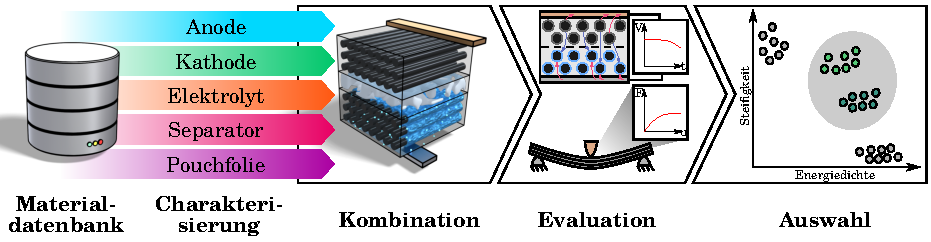
\includegraphics[width=\textwidth, angle=0]{methode.pdf}
		\caption{\label{fig:own_methode}Im Rahmen der Arbeit entwicklete Methode zur Identifizierung von neuen anwendungsspezifischen Strukturbatterien.}
\end{figure}

Die Erarbeitung dieser effizienteren multiphysikalischen Modelle stellen dabei den Ausgangspunkt dieser Arbeit dar. Dabei liegt ein großer Fokus auf der Berücksichtigung auf dem Einfluss von herkömmlichen Elektrolyten und Strukturelektrolyten auf Energiedichte- und Steifigkeitsbetrachtungen. Die Modelle werden anschließen in einem digitalen Framework implementiert. Im Weiteren werden die benötigten Parameter aus der bestehenden Literatur und eigenen Experimenten ermittelt und in einer eigens erstellte Materialdatenbank gesammelt. Aus den verschiedenen Materialien werden durch geeignte Vorauswahlmechanismen die Menge an denkbaren Konfigurationen eingeschränkt. Anschließend wird für jede verbleibende Konfiguration evaluiert und auf ihrer Einsatzszenarien abgeleitet. %Im dritten Schritt werden potenzielle Strukturspeicher mithilfe der validierten Einzelmodelle bewertet und exemplarisch an ausgewählten Kandidaten überprüft. 
Abschleißend werden die bei der Analyse als äußerst vorteilhaften Material- und Parameterkombinationen durch Experimente erprobt und somit eine abschließende Validierung der Methodik erbracht. % dienten \textsc{Kühn} und \textsc{Seidel-Greiff} als Grundlage für ihre experimentellen Untersuchungen, die in der prototypischen Fertigung einer Strukturbatterie kulminierten.

%Mithilfe der entwickelten Methode konnte eine optimierte Strukturbatterie für einen hybriden Anwendungsfall identifiziert werden. Ein erster Funktionsprototyp zeigte eine xx~\% höhere multifunktionale Performanz gegenüber bisher veröffentlichten Strukturbatterien.

% Das zugrundeliegende Prinzip dieses Lösungsansatzes besteht darin, dass Computer besser dazu geeignet sind, eine Vielzahl von einfachen Zusammenhängen zu verarbeiten und dies wiederholt für jede erdenkliche Kombination anzuwenden. Im Gegensatz zu bestehenden Ansätzen beginnt die Modellierung nicht auf atomarer Ebene, sondern auf der Komponentenebene, was eine schnellere Generierung von Ergebnissen ermöglicht. Zudem kann das Modellsystem leicht um Modelle auf mikro- oder molekularer Ebene erweitert werden, um zusätzliche Einflussfaktoren zu berücksichtigen.


%**************************************************************
%                   LITERATURÜBERSICHT  
%**************************************************************
\section{\label{sec:Literaturübersicht}Literaturübersicht}
% 3-5 Seiten

\subsection*{Existierende Strukturbatteriekonzepte}

\begin{figure}[ht]
	%\raggedleft
		%\def\svgwidth{\columnwidth}
        \center
	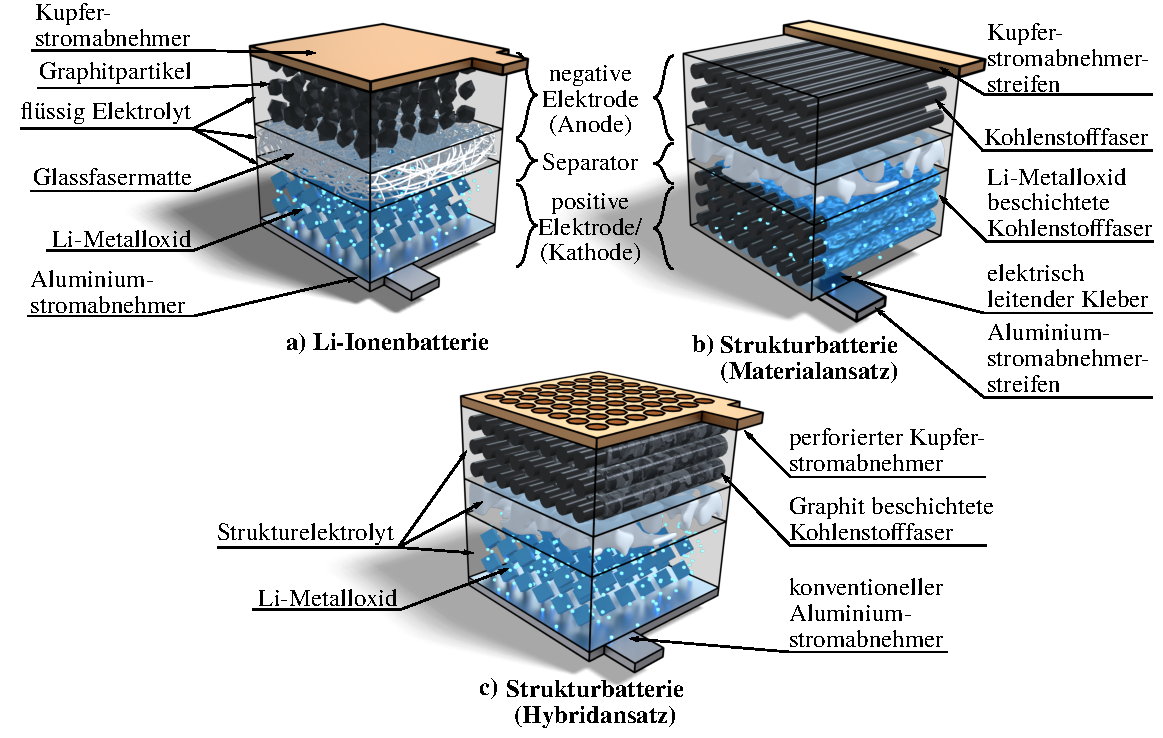
\includegraphics[width=\textwidth, angle=0]{sb_types.pdf}
		\caption{\label{fig:sb_types}Vereinfachte Darstellung von a) konventionellen Li-Ionen Batterie, b) einer Strukturbatterie als multifunktionales Material und c) als multifunktionale Struktur.}
\end{figure}

Die erste multifunktionale Strukturbatterie wurde 2004 von \textsc{Wetzel} et al. im Army Research Laboratories (ARL) der USA entwickelt \cite{Wetzel2004, Snyder2006, Wong2007, Snyder2007}. Die Strukturbatterie Verbundmaterialien basierten auf Kohlenstofffasern als Anode, einer mit $\text{LiFePO}_\text{4}$ beschichteten Edelstahlkathode und einer Glasfasermatte als Separator \cite{Wong2007}. Dieser Aufbau zeigte bereits gute mechanische Eigenschaften. Allerdings konnten die elektrochemischen Eigenschaften wegen auftretender Kurzschlüsse nicht abschließend bestimmt werden.

2009 konzeptionierten \textsc{Liu} et al. \cite{Liu2009} die erste kurzfaserverstärkte Elektrode mit einem festen Polymerelektrolyt als Matrixmaterial. Allerdings konnte die faserverstärkte Elektrode nicht herstellt werden und keinen Feststoffelektrolyten mit ausreichender Ionenleitfähigkeit gefunden werden, weshalb schließlich auf ein gelbasiertes Elektrolyt mit festen und flüssigen Phasenanteilen umgeschwenkt wurde. Da aufgrund der besseren Ionenleitfähigkeit weniger Elektrolyt eingesetzt werden musste, konnte eine Energiedichte von 35~$\si{\watt \hour \per \kg}$ erreicht werden. Durch die fehlende strukturelle Verstärkung wurde allerdings nur ein geringer E-Modul von 3~GPa erreicht.

Der Ansatz der Verwendung von Gelelektrolyten wurde von \textsc{Ekstedt} et al. verfolgt \cite{Ekstedt2010}, in das erstmals ein Kohlenstofffasergewebe als Elektrode einbettet wurde. Ähnlich wie in den Arbeiten von \textsc{Wetzel} et al. wurde auch hier ein glasfaserbasierter Separator und eine mit $\text{LiFePO}_\text{4}$ beschichtete, gewebte Aluminiumfasermatte als Kathode verwendet. Die resultierende Batterie zeichnete sich durch eine Zellspannung von 3,3~V aus. Allerdings wurden die mechanischen und elektrochemischen Eigenschaften nur theoretisch ermittelt.

Im Jahr 2011 präsentierten \textsc{Carlson} et al. \cite{Carlson2011} eine der ersten funktionierenden Strukturbatterien mit einer laminatartigen Struktur. Diese bestand aus einem IMS65-Kohlenstofffasergewebe als Anode, einem Gelelektrolyt, einem Glasfaserseparator und einer mit $\text{LiFePO}_\text{4}$ beschichteten gewebten Aluminiumfolie. Die speicherbare elektrische Energie betrug 0,0247~$\si{\watt \hour \per \kg}$, was ausreichte, um eine LED 70~s lang zu einem schwachen Leuchten zu bringen.

Zwei Jahre später wurden \textsc{Asp} et al. \cite{Asp2013US,Asp2013CN} zwei Patente zugesprochen, die einen Ansatz beschreiben, durch gezielte Funktionalisierung der Faseroberflächen jede Kohlenstofffaser zu einer Elektrode zu machen. Auch wenn die Patente seit 2017 nicht mehr verfolgt werden, wurde darauf aufbauend eine Batterie entwickelt, mit der eine Energiedichte von 10~$\si{\watt \hour \per \kg}$ erzielt wurde. Die theoretisch möglichen 175~$\si{\watt \hour \per \kg}$ bei einem gleichzeitigen Schubmodul von 1~GPa wurden jedoch noch nicht ansatzweise erreicht \cite{Leijonmarck2013, Carlson2013}.

2018 untersuchte \textsc{Meng} et al. \cite{Meng2018} erstmalig den Einsatz von vertikal ausgerichteten Karbonnanoröhrchen (CNT). Diese wurden für die Elektrode auf ein Edelstahlnetz aufgedampft. Anschließend wurde für die Anode $\text{NiO}_\text{x}$ durch einen elektrochemischen Ausscheidungsprozess auf die CNT-Edelstahlelektrode eingelagert. Mit dem gleichen Verfahren wurde $\text{FeO}_\text{x}$ für die Kathode aufgetragen. Die Strukturbatterie erreichte dabei eine Zugsteifigkeit von 7,0~GPa und eine Energiedichte von 1.4~$\si{\watt \hour \per \kg}$.

\textsc{Moyer} et al. \cite{Moyer2020} modifizierten den für Batterien typischen Pouchzellenansatz, indem das verpresste Kohlenstofffasergewebe gleichzeitig als Stromkollektor und Schutzfolie dient. Durch das anodenseitige Aufbringen von Graphit und $\text{LiFePO}_\text{4}$ auf der Kathode nehmen die Fasern jedoch nicht direkt am chemischen Prozess teil. Durch das bessere, als Interkalation bezeichnete, Ionen-Einlagerungsverhalten bei Graphit konnte eine hohe Energiedichte von 35~$\si{\watt \hour \per \kg}$ gemessen werden. Jedoch führte der Ansatz zu einer vergleichsweise geringen Zugsteifigkeit von 2~GPa.

\textsc{Thakur \& Dong} \cite{Thakur2020} stellten 2020 die erste 3D-gedruckte Strukturbatterie her. Mithilfe eines Koextrusionsprozesses konnte eine Kohlenstofffaser, die vorher mit einem festen Polymerelektrolyten beschichtet wurde, zusammen mit einem Li-gedopten Polylactide-Matrixmaterial aufgebracht werden. Nach dem Drucken der Elektrode wurde manuell eine Glasfasermatte und abschließend eine Aluminiumfolie als Kathode aufgebracht. Neben der Möglichkeit, neue Batteriegeometrien zu drucken, wurde auch durch die höhere Dichte an Aktivmaterial in Fasernähe eine vergleichsweise hohe Energiedichte von 24~$\si{\watt \hour \per \kg}$ erreicht. Allerdings konnte durch den geringen Faservolumenanteil ein niedriges Zugmodul von 0.29~GPa gemessen werden.

2021 präsentierte \textsc{Asp} et al. \cite{Asp2021} ein Design mit unidirektionalen Kohlenstofffasern als Anode, einem gewebten Glasfaserseparator und einer $\text{LiFePO}_\text{4}$-beschichteten Aluminiumplatte als Kathode. Durch ein verbessertes Herstellungsverfahren und eine günstige Faseranordnung konnte ein E-Modul von 25~GPa und eine Zugfestigkeit von 300~MPa gemessen werden. Gleichzeitig erreichte die Strukturbatterie eine Energiedichte von 24~$\si{\watt \hour \per \kg}$. \textsc{Siraj} et al. \cite{Siraj2023} verbesserten zwei Jahre später den Infiltrationsprozess, wodurch sie bei annähernd gleichbleibenden mechanischen Eigenschaften die Energiedichte auf nahezu 41~$\si{\watt \hour \per \kg}$ verdoppeln konnten.

\begin{table}[ht]
    \centering
    \caption{Auswahl realisierter Strukturbatterien}
    \begin{tabular}[t]{m{0.15\textwidth} m{0.15\textwidth}<{\centering} m{0.15\textwidth}<{\centering} m{0.2\textwidth}<{\centering} m{0.1\textwidth}<{\centering} m{0.1\textwidth}<{\centering}}
    \toprule
    &Elastizitäts-modul~[GPa]&Energie-dichte~[Wh/kg]&Struktur-batterieart&Jahr&Referenz\\
    \midrule
    \textsc{Wong et al.}&8&/&Edelstahlbatterie&2007&\cite{Wong2007}\\
    \textsc{Liu et al.}&3&35&Faserbatterie&2009&\cite{Liu2009}\\
    \textsc{Meng et al.}&7&4&Edelstahlelektroden&2018&\cite{Meng2018}\\
    \textsc{Moyer et al.}&35&2&Kohlenstofffaser-verbund&2020&\cite{Moyer2020}\\
    \textsc{Thakur et Dong}&0.29&24&Faserbatterie&2020&\cite{Thakur2020}\\
    \textsc{Huang et al.}&9.2&43&Edelstahlelektroden&2020&\cite{Huang2020}\\
    \textsc{Asp et al.}&25&24&Kohlenstofffaser-verbund&2021&\cite{Asp2021} \\
    \textsc{Saraj et al.}&26&41&Kohlenstofffaser-verbund&2023&\cite{Siraj2023}\\
    \bottomrule
    \end{tabular}
\end{table}%

Die existierenden Studien an Strukturbatterien zeigen einen starken Fokus auf geschichtete Bauweisen, die sich an die Struktur von herkömmlichen Lithiumionenbatterien anlehnt, siehe Bild~\ref{fig:sb_types}a,b. Aus den bisherigen Ergebnissen leiten sich außerdem eine Reihe an Verbesserungspotenzialen für weitere Forschungen ab. Die größte Herausforderung stellt bislang das Erzielen einer möglichst guten Lithium-Interkalation in das Aktivmaterial der Elektrode dar. Das Gleiche gilt für die Lithiummigration zwischen den beiden Elektroden über den Strukturelektrolyt, welche möglichst unbehindert, bei gleichzeitiger Beibehaltung der mechanischen Steifigkeit und Festigkeit,  stattfinden muss~\cite{Asp2015}. Besonders zur weiteren Eröhung der Energiedichte, sind neue Ansätzte wie perforierte Stromabenehmer, Seperatorfreie Bauweisen durch Strukturelektorlyt oder hybride Bauweisen für bessere zellchemie denkbar, siehe Bild~\ref{fig:sb_types}c. Die Wichtigkeit solcher Verbesserungen wird dadurch verstärkt, dass die aktuell höchste erreichte Energiedichte von 41~$\si{\watt \hour \per \kg}$ am unteren Ende der benötigten Energiedichte, die für den Einsatz in z.B. Elektrofahrzeugen erforderlich ist, liegt. Diese Mindestgrenze der Energiedichte wurde allerdings 2022 von dem Forschungsteam um \textsc{Linde} am Deutschen Zentrum für Luft- und Raumfahrt (DLR) weiter angehoben auf 74~$\si{\watt \hour \per \kg}$, bei einem gleichzeitig Mindest-E-Modul von 54~GPa und einer Mindestfestigkeit von 203~MPa, sowie einer Leistungsdichte von 376~W/kg ~\cite{Ishfaq2022}. Womit ein Durchbruch für Strukturbatterien im Sinne einer industriellen Anwendung noch aus steht.

\subsection*{Modellierung des gekoppelten elektrochemischen und mechanischen Verhaltens von Strukturbatterien}

Über jedes Material was in einer heutigen sicherheitsrelevanten Anwendung verwendet wird muss ausreichendes Wissen existieren um das Verhalten im Belastungsfall ausreichend vorherzusagen. Bei Strukturbatterien besteht die Herausforderung nicht sowohl die elektrochemsichen und mechansichen Prozesse einzeln zu verstehen, sondern auch dabei ihre gegenseitigen Wechselwirkungen zu berücksichtigen~\cite{Carlstedt2022a}. Diese Schwierigkeiten werden durch den hohen Multifunktionalitätsgrad von Material und Struktur zu einem .

Eine vergleichsweise einfache Beschreibung der elektrochemischen und thermischen Phänomenen kann durch äquivalente Ersatzschaltungen (\textit{engl.} equivalent circuit model, ECM) erfolgen \cite{Bavsic2022}. Bereits mit wenigen Elementen lassen sich Spannungsänderungen in Abhängigkeit vom Lade- und Entladeverhalten gut annähern \cite{YannLiaw2004}. Durch zusätzliche Erweiterungen lassen sich auch Alterung und der Einfluss zahlreicher thermischer Effekte berücksichtigen \cite{Hannan2017,Tran2021}. Aufgrund des geringen Rechenaufwands eignen sich diese Modelle besonders gut für zeitkritische Anwendungen wie die Lade- und Entladeregelung, siehe Abbildung~\ref{fig:battery_modelling_in_context}. Die Modellparameter müssen jedoch jedes Mal durch einen Fittingprozess für das jeweilige System bestimmt werden \cite{Tomasov2019}. Eine Verknüpfung der einzelnen Schaltelemente mit realphysikalischen Größen war bisher nur wenig erfolgreich \cite{Plett2015}.
\begin{figure}[ht]
	%\raggedleft
		%\def\svgwidth{\columnwidth}
        \center
	\includegraphics[width=\textwidth, angle=0]{batterie_modelling_approaches.pdf}
		\caption{\label{fig:battery_modelling_in_context}Übersicht der Batteriemodellierung im Kontext neuer Batterieentwicklungen.}
\end{figure}
Die physikalische Modellierung der elektrochemischen Phänomene wurde maßgeblich von \textsc{Doyle} \cite{Doyle1995,Doyle2003,Ceder2002}, \textsc{Fuller} \cite{Fuller2018,Takeuchi2008} und \textsc{Newman} \cite{Doyle1995,Newman2021} vorangetrieben. Das von ihnen entwickelte und nach ihnen benannte DFN-Modell (alternativ auch \textit{pseudo zwei dimensionale} (P2D) Modell genannt) \cite{Doyle1993} beschreibt die Prozesse auf der Makroskala und eignet sich daher sehr gut, um die Vorgänge auf Zellebene zu modellieren. Die benötigten Parameter können durch Experimente oder mithilfe von Simulationen auf niedrigeren Skalen wie der Dichtefunktionaltheorie (DFT) oder molekulardynamischen (MD) Simulationen bestimmt werden \cite{Chen2022}. Das DFN-Modell findet heute weitreichenden Einsatz und wurde seit seiner Veröffentlichung im Jahr 1993 zahlreich modifiziert und erweitert. Einige der bekanntesten Derivate sind das \textit{Single Particle Model} (SPM) \cite{Li2017} und das \textit{full homogenized macro-scale} (FHM) Modell \cite{Arunachalam2019}, welche beide darauf abzielen, die sehr rechenintensiven Differentialgleichungen in ihrer Komplexität zu reduzieren.

Die Kopplung mit thermischen Prozessen wurde bereits 1995 von \textsc{Pals et Newman} \cite{Pals1995,Pals1995a} begonnen und seitdem kontinuierlich weiterentwickelt \cite{Chen2005,Onda2006,Kim2013,Gao2021,Liu2023}. Auch der Einfluss der lithierungsbedingten Ausdehnung \cite{Bower2011,Yang2014,Roberts2014,Pereira2019,Mai2019,Li2020,Hoeschele2023}, Rissbildung \cite{Dionisi2017,Wang2020a,Pistorio2023} und Alterung \cite{RedondoIglesias2020} wurden in zahlreichen Studien untersucht. Zusätzlich existieren viele Studien, die sich einer vereinheitlichten Modellierung aller Effekte \cite{Wu2014,Kim2018,Liu2020,Yin2020} und auch einer Modellierung über mehrere Größenskalen hinweg widmen \cite{Liu2019,Li2020a,Katrasnik2021}.

\textsc{Carlstedt} erarbeitete stückweise in einer Reihe von Beiträgen eine Koppelung von Elektrochemie, Mechanik und Thermodynamik, um das Verhalten von Strukturbatterien zu beschreiben \cite{Carlstedt2019,Carlstedt2019a,Carlstedt2019b,Carlstedt2020,Carlstedt2020b,Carlstedt2022,Carlstedt2022a,Carlstedt2022b}. Auch wurde der Ansatz um den nicht-linearen Zusammenhang durch die Gestaltänderung von \textsc{Larsson} et al. \cite{Larsson2023} erweitert.

\subsection*{Modelierungsgetriebene Entwicklung von neuen Batterien und Strukturbatterien}

Die neu motivierte Forschung in bereits untersuchte und neue Batteriematerialien baut aktuell hauptsächlich auf theoretischen Überlegungen und experimentellen Prototypen auf. Um die Vielzahl an Effekten zu berücksichtigen und der enormen Anzahl an vielversprechenden Materialkombinationen Herr zu werden, argumentierten \textsc{Greenhalgh} \cite{Greenhalgh2024,Greenhalgh2024a} und \textsc{Asp} \cite{Asp2024} auf dem \textsc{1st Structural Power Research Showcase} in London, dass nur durch intensive Modellierungsarbeit diese Varianten voruntersucht und ausreichend eingeschränkt werden können. Der multiphysikalische Modellierungsansatz von \textsc{Carlstedt} wird zwar in diesem Zusammenhang oft erwähnt, allerdings sorgen Skalierungseffekte, wie etwa Defekte und Faser-Matrix-Interfaceeffekte, die besonders bei Oberflächenmodifikation von Kohlenstofffasern sowohl für deutlich andere elektrochemische als auch mechanische Eigenschaften des Verbundes sorgen, für große Ungenauigkeiten bei der Adaption \cite{Franco2019,Fam2024}. Hinzu kommt, dass die Modelle von Carlstedt mit zunehmender Komplexität immer mehr Materialparameter benötigen und bereits jetzt mehr als 20 teils aufwendig zu bestimmende Parameter pro Material erfordern \cite{Greenhalgh2024a}. Bis heute wurde dieser Ansatz daher vor allem zur nachträglichen Validierung und zur detaillierten Untersuchung von sensorischen und aktuatorischen Effekten von Strukturbatterien genutzt \cite{Carlstedt2023}.

Die einzige zurzeit existierende Veröffentlichung zur Vorhersage von Energiedichte und Zugsteifigkeit stammt ebenfalls von \textsc{Carlstedt} \cite{Carlstedt2018}. Jedoch wurde dazu ein in der Komplexität deutlich reduzierter Ansatz verwendet. Hinzu kommt, dass bei der Auswertung nur drei Varianten untersucht wurden, die sich in ihrer Elektrodendicke und dem Volumenanteil des Aktivmaterials unterschieden. Außerdem wurde der Einfluss des Elektrolyten nicht berücksichtigt.



% Dan Zenkert KTH Prof (Fasercehmie), 
% Dr Faye Smith OBE (Director at Avalon Consultancy Services)
% Peter Linde (DLR, CORCER Mitgleid)
% Milo Shaffer ( Professor of Materials Chemistry London)
% Natasha Shirshova (Lecturer in Engineering Materials at Durham University)
% Derrick Fam (Scientist at Institute of Materials Research and Engineering (IMRE), Adjunct Assistant Professor (NTU, MSE), Dy. Dir. Singapore Battery Consortium)
% Alexander Bismarck (Professor of Material Chemistry Wien)
% Madhavi Srinivasan (Professor at Nanyang Technological University Singapore)



   


\chapter{Stand der Forschung}

Im folgenden Kapitel wird ein grundlegendes Verständnis für die Funktionsweise von Strukturbatterien vermittelt. Außerdem werden die Besonderheiten im Vergleich zu konventionellen Batterien und faserverstärkten Verbundwerkstoffen erläutert. Dazu werden die wichtigsten Eigenschaften und deren Ermittlungsverfahren dargestellt sowie die Rolle der einzelnen Komponenten im Zusammenhang mit der Materialauswahl näher erklärt. Anschließend werden aktuelle Entwicklungsansätze diskutiert und abschließend die ungelösten Herausforderungen mit den aktuellen Methoden näher analysiert.

\section{Funktionsweise der Strukturbatterie} Strukturbatterien sind Batterien, die mechanisch belastbar sind und damit auch zur strukturellen Integrität beitragen können.
Batterien erlauben es, temporär Energie zu speichern, indem Ladungsträger reversibel in einem Hostmaterial eingelagert werden. Solche Zellen werden daher auch ''Shuttle-Clock''~\cite{Ohzuku1993}-, ''Rocking-Chair''~\cite{Tarascon1993}- oder ''Swing''~\cite{Bittihn1993}-Zellen genannt. Der Einlagerungsprozess selbst wird meist als ''Interkalation'' bezeichnet~\cite{Eichinger1976}. Durch den Einlagerungsprozess nehmen die beiden Hostmaterialien aktiv am Ladungsaustausch teil, daher auch der Name ''Aktivmaterial'', siehe Bild~\ref{fig:battery_function}. Häufig ist das Aktivmaterial für die Anode Graphit und für die Kathode ein Metalloxid (\ce{MO_2}).
\begin{figure}[h]
	%\raggedleft
		%\def\svgwidth{\columnwidth}
        \center
	\includegraphics[width=\textwidth, angle=0]{battery_function.pdf}
		\caption{\label{fig:battery_function}Die Energiespeicherfunktion einer Batterie wird maßgeblich durch den skalenübergreifenen Ein- und Auslagerungsprozess der Ladungsträger realisiert.}
\end{figure}
Beim Entladen der Batteriezelle wandern die Ladungsträger von der Anode zur Kathode. An beiden Elektroden kommt es zum Ladungsaustausch, der mittels Redox-Gleichungen beschrieben werden kann~\cite{Goodenough2013}: 
\begin{align}
	\ce{C_6 + x Li^+ + x e^- &<=> Li_xC_6}\\ 
	\ce{LiMO_2 - x Li^+ - x e^- &<=> Li_{1-x}MO_2} 
\end{align} 
Der Einlagerungsprozess erlaubt im Vergleich zur reinen elektrostatischen Speicherung, wie etwa bei Kondensatoren, eine signifikant höhere Beladungsdichte an Ladungsträgern, wodurch größere Energiemengen gespeichert werden können~\cite{Newman2021}.

Entscheidend für die Funktion der Batterie ist hierbei, dass der Transport der Ionen durch den Elektrolyten und den Separator erfolgt. Die Elektronen können jedoch nur entlang des Stromkollektors geleitet werden und müssen daher einen „Umweg“ außerhalb der Zelle machen~\cite{Plett2015}, siehe Bild~\ref{fig:battery_function}. Die Bewegung der Elektronen ist dabei im Vergleich zum Ionentransport deutlich schneller, weshalb die Ent- und Beladungsgeschwindigkeit einzig von der Ionenmobilität limitiert wird~\cite{Plett2024}.

Im Falle großer Ströme, wie etwa bei einem Kurzschluss, finden viele Ladungsumwandlungsreaktionen gleichzeitig statt. Die dabei entstehende Wärme kann zum Versagen oder Brennen der Zelle führen. Mögliche Ursachen für Kurzschlüsse sind Herstellungsfehler, Dendritwachstum und mechanische Belastungen, bei denen die Elektroden durch Versagen des Separators in direkten Kontakt kommen, wie etwa bei Penetration oder Biegung~\cite{Beard2019}.

Darüber hinaus führt die mit den mechanischen Belastungen einhergehende Rissbildung zu einer Erhöhung des inneren elektrischen Widerstandes, was zu einem Verlust an Speichereffizienz führt und daher vermieden werden soll~\cite{Plett2024}. Bei konventionellen Batterien kommen daher spezielle Umhausungen zum Einsatz, die eine Belastung der Batterien verhindern sollen~\cite{Beard2019}. Diese bringen allerdings einen signifikanten Anteil an zusätzlicher Masse hinzu und sind aufgrund ihrer Größe meist schwerer in Hoststrukturen zu integrieren~\cite{Asp2021}. Um diesen Nachteilen zu begegnen, versuchen Strukturbatterien durch die Integration geeigneter Materialien die mechanische Belastungsfähigkeit zu verbessern~\cite{Carlstedt2018}. Zur Steigerung der Multifunktionalität neuer Strukturbatterien ist daher neben einem umfangreichen Verständnis der wichtigsten Eigenschaften auch ein Überblick über mögliche Materialkandidaten aus bestehenden Untersuchungen zu konventionellen Batterien sowie dem Leichtbaubereich notwendig~\cite{Asp2019}.


\section{Wichtigsten Eigenschaften und ihre Ermittlungsverfahren}
%\subsection{Interkalation}
\subsection{Ladungszustand}
Ein wesentliches Merkmal von Batterien ist die Einlagerung von Ionen in das Hostmaterial (Interkalation). Je nach Hostmaterial steht dabei eine bestimmte Menge an Einlagerungsplätzen zur Verfügung. Der Ladungszustand (\textit{engl.} state of charge, SOC) beschreibt den Anteil der besetzten Plätze an den insgesamt verfügbaren Plätzen~\cite{Plett2015}.

Das bedeutet, dass, wenn alle Plätze belegt sind, der SOC gleich 1 bzw. 100~\% ist, und wenn alle Ionen das Hostmaterial verlassen haben, also keiner der Plätze belegt ist, der SOC einen Wert von 0~\% hat. Alternativ wird der Beladungszustand auch durch die stöchiometrische Größe $x$ angegeben, die besonders häufig im Kontext der Beschreibung von Zwischenzuständen (z.B. \ce{Li_xMn2O4} oder \ce{Li_{1-x}C}) benutzt wird~\cite{Newman2021}. Der SOC hat maßgeblichen Einfluss auf das chemische Potenzial (siehe Bild~\ref{fig:battery_voltage}), die Volumenausdehnung (siehe Tabelle~\ref{tab:volume_change}) und die Diffusionsgeschwindigkeiten~\cite{Plett2024}. Der SOC kann jedoch nicht direkt gemessen werden und wird stattdessen über die Elektrodenspannung ermittelt~\cite{Newman2021}.

\begin{table}[ht]
    \centering
    \caption{\label{tab:volume_change}Volumenänderungen bo der Lithiierung für gängige Aktivmaterialien.}
    \begin{tabular}[t]{lccc}
        \toprule
        Material& Volumenänderung $\Delta$V/V\textsubscript{0}&Verlauf&Referenz\\
        \midrule
        Graphit & +10\% - +13\% & nicht-linear & \cite{Qi2010,Woodford2012}\\
        NMC111 &-2,4\%&nicht-linear& \cite{Yabuuchi2005}\\
        NMC422 &+2,4\%&nicht-linear& \cite{Ma2007}\\
        LCO &-1,9\% & linear & \cite{Reimers1992}\\
        NCA &-1,6\% & nicht-linear& \cite{Itou2005}\\
        LFP &+6,5\% & linear & \cite{Padhi1997}\\
        LMO &+6,6\% & linear & \cite{Christensen2006}\\
        \bottomrule
    \end{tabular}
\end{table}

\subsection{Elektrische Spannung}

Die elektrische Spannung ist neben dem Strom, der direkt mit der Bewegung der Ladungsträger verbunden ist, eine der wichtigsten Größen zur Beschreibung des Zustandes in einer Batteriezelle~\cite{Beard2019}. 

\begin{figure}[h]
    \center
		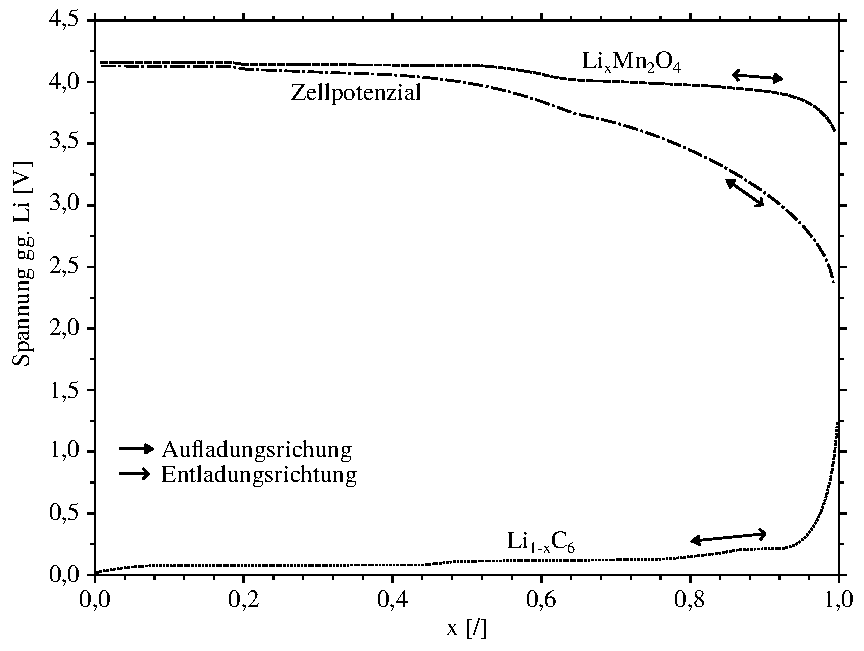
\includegraphics[width=\textwidth, angle=0]{uocp.pdf}
		\caption{\label{fig:battery_voltage}Spannung über den stöchiometrischen Anteil der beladung einer Lithiumionenbatterie, sowie die Anteile der negativen (Graphit) und positiven (Manganoxid) Elektrode (angelehnt an~\cite{Newman2021}).}
\end{figure}

Im Kontext der Elektrochemie ist die elektrische Spannung ein Maß für das elektrochemische Potenzial einer Elektrode. Ein Potenzial kann jedoch nur durch den Vergleich zu einem Referenzpotenzial, das dann oft als ''Nullpotenzial'' bezeichnet wird, gemessen werden. In der Batterieforschung wird hierbei häufig die Referenzspannung gegen reines Lithium gemessen~\cite{Newman2021}. Entscheidend ist hierbei, dass diese Referenzspannung bei einer Elektrode nicht konstant ist, da sich durch das Ein- und Auslagern das chemische Potenzial verändert. Der resultierende Funktionsverlauf ist abhängig von der chemischen Struktur und kann damit Aufschlüsse auf das Einlagerungsverhalten und damit verbundene Phasenumwandlungen geben~\cite{Plett2015}, siehe Bild~\ref{fig:battery_voltage}.

Damit Batterien sich nicht selbst entladen, wenn ein Verbraucher angeschlossen ist, ist es wichtig, dass die Zellspannung, auch als nominale Spannung bezeichnet, mit zunehmender Entladung stetig sinkt~\cite{Newman2021}, siehe Bild~\ref{fig:battery_voltage}. Der reversible Lithiumbeladungsprozess ist dabei stets mit einem abnehmenden Potenzialanstieg an der jeweiligen Elektrode verbunden. Da in einer Batterie durch den Ladungsaustausch immer eine Elektrode beladen wird, während die andere entladen wird, kann der stetige Spannungsabfall während der Entladung sichergestellt werden, wenn die Referenzspannung einer Elektrode immer größer ist als die der anderen~\cite{Plett2024}. Aus dem stetigen Verlauf der Zellspannung leiten sich für die Anwendung weitere wichtige Spannungsgrößen ab: die Abschaltspannung, die die minimal erlaubte Spannung und damit den ''entladenen'' Zustand markiert~\cite{Plett2015}.

Eine weitere wichtige Kenngröße für Batterien ist die Leerlaufspannung, welche gemessen wird, wenn kein Strom zwischen den beiden Elektroden fließt. Daher ist sie von signifikanter Bedeutung für die Beschreibung des Gleichgewichtszustandes innerhalb der Zelle~\cite{Newman2021}.

\subsection{C-Raten}
Die Auflade- oder Entladerate einer Batterie wird oft in sogenannten C-Raten angegeben. Dabei bedeutet 1~C, dass eine vollständig entladene/geladene Batterie in 1~h komplett aufgeladen/entladen wird. Bei einer doppelt so hohen C-Rate wird die Batterie folglich in der Hälfte der Zeit, also 30~min, entladen bzw. aufgeladen. Bei einer halb so hohen Auflade- bzw. Entladerate (0.5C oder C/2) benötigt die Batterie 2~h, um vollständig aufgeladen oder entladen zu werden. Die Wahl der C-Rate ist vor allem bei der Messung der Kapazität von Bedeutung. Verallgemeinert gilt: Je höher die C-Rate, desto geringer ist die gemessene Kapazität. Die Stärke des Kapazitätsabfalls wird durch eine Reihe von Faktoren, wie Übergangsverhalten, Form und Art der chemischen Struktur der Elektrode usw., bestimmt~\cite{Plett2015,Beard2019}.


\subsection{Kapazität}
Die Kapazität einer Elektrode beschreibt, wie viele Ladungsträger eingelagert oder entfernt werden können. Besonders in den ersten Zyklen ist der Unterschied zwischen Auflade- ($\text{C}_{\text{aufl}}$) und Entladekapazität ($\text{C}_{\text{entl}}$) signifikant, weshalb die Kapazität für beide Prozesse getrennt bestimmt wird~\cite{Plett2015}.

Zur Ermittlung der Kapazität wird ein konstanter Auflade- ($\text{I}_\text{C,aufl}$) oder Entladestrom ($\text{I}_\text{C,entl}$) (C-Rate) an eine Zelle aus Elektrode und Referenzelektrode, meist Lithiummetall, angelegt und die Zeit $\Delta \text{T}_\text{aufl}$ gemessen, die für die komplette Auf- bzw. Entladung benötigt wird. Da die Kapazität das zeitliche Integral des Stromes ist, kann die Bestimmung auf die folgenden Formeln vereinfacht werden~\cite{Newman2021}:
\begin{align}
	\text{C}_{\text{aufl}} &= \text{I}_\text{C,aufl} \cdot \Delta \text{T}_\text{aufl}\\
	\text{C}_{\text{entl}} &= \text{I}_\text{C,entl} \cdot \Delta \text{T}_\text{entl}.
\end{align}

%komplett entladen oder in der die Spannung von Abschalt- bzw. Leerspannung $\text{U}_{\text{leer}}$ zur vorher ermittelten maximal Spannung $\text{U}_{\text{voll}}$ benötigt. Die Aufladekapazit stellt dabei das Produkt aus Durch Umkehrung des Prozesses lässt sich die Entladekapazität bestimmen 

Bei der Entwicklung neuer Batteriematerialien wird die Kapazität meist auf die Masse des am Einlagerungsprozess teilnehmenden Materials (Aktivmaterial) normiert. Diese spezifische Kapazität hat dann die Einheit [$\si{\A \hour \per \g}$]. Im Kontext der Batterieentwicklung wird allerdings die Kapazität je Elektrodenfläche [$\si{\A \hour \per \cm\squared}$] häufig angegeben.


\subsection{Columbische Effizienz}
Die coulombsche Effizienz (CE) ist eine der meistbenutzten Metriken, um die interne Reaktion zu bewerten. Die CE des Zyklus \( n \) ist definiert als das Verhältnis der gemessenen Kapazität während des Entladevorgangs \( C_{Dch}(n) \) zur Kapazität des vorherigen Beladungsvorgangs \( C_{Ch}(n) \) \cite{Tornheim2020}.
Die Formel
\begin{equation}
CE = \frac{C_{Dch}(n)}{C_{Ch}(n)}
\end{equation}
gilt dabei für Aufbauten, die in einem Entladenzustand zusammengebaut werden und daher zuerst beladen werden müssen. Zellen, die in einem beladenen Zustand gefertigt werden, wie etwa Lithium-Schwefel-Batterien, beginnen allerdings zuerst mit einem Entladungszyklus. Die korrekte Formel lautet in einem solchen Fall
\begin{equation}
    CE = \frac{C_{Dch}(n+1)}{C_{Ch}(n)}.
\end{equation}

\subsection{Kapaziätserhalt}
Die Kapazitätserhalt (\textit{engl.} Capacity Retention) ist eine wichtige Metrik, um den Anteil an Nebenreaktionen, die zu einem Kapazitätsverlust in Batterien führen, zu bemessen. Sie ist definiert als das Verhältnis von Entladungskapazität des $(n+1)$-ten Zyklus $C_{Dch}(n+1)$ und der des $n$-ten Zyklus $C_{Dch}(n)$:
\begin{equation}
    CE = \frac{C_{Dch}(n+1)}{C_{Dch}(n)}.
\end{equation}
In einigen Fällen wird CR auch im Verhältnis zur initialen Entlade-Kapazität bestimmt, also
\begin{equation}
    CE = \frac{C_{Dch}(n)}{C_{Dch}(1)}.
\end{equation}
Dieser Ansatz ist besonders dann hilfreich, wenn die Langlebigkeit zu bestimmen ist \cite{Tornheim2020}.
Im Gegensatz zu CE ist CR meist relevanter für Hersteller und Endnutzer.

\subsection{Energiedichte}
Die gravimetrische Energiedichte bzw. spezifische Energie bemisst, wie viel Energie pro eingesetzter Masse gespeichert werden kann. Alternativ wird mittels der volumetrischen Energiedichte die Menge an speicherbarer Energie pro Volumen angegeben. Beide Kenngrößen sind wichtige Größen, die bei der Entwicklung neuer Speichertechnologien nach Möglichkeit gesteigert werden sollen~\cite{Plett2015}.

Eine der größten Schwierigkeiten beim Umgang mit angegebenen Energiedichten aus der Literatur besteht in dem Umstand, dass oft bei der Masse oder dem Volumen auf verschiedene Komponenten Bezug genommen wird~\cite{Son2021}. Im Allgemeinen unterscheiden sich die Angaben darin, ob die Werte im Kontext von:
\begin{enumerate}
	\item Materialentwicklung
	\item Elektrodenentwicklung
	\item Zellentwicklung
\end{enumerate}
erhoben wurden, siehe Tabelle~\ref{tab:energy_densities}.
So wird bei der Forschung an neuen Aktivmaterialien die spezifische Energie auf die eingesetzte Masse an Aktivmaterial bezogen. Im Bereich neuer Elektroden wird die Speicherkapazität entweder auf die Elektrodenmasse oder, im Falle einer Oberflächenbeschichtung, meist nur auf die Masse der Beschichtung normiert. In Publikationen zu neuen Zellen gibt es noch mehr Varianten. Je nach Autor finden sich hier Angaben in Referenz zur Masse der gebauten Knopfzelle oder der gebauten Pouchzelle; bei Letzterer gibt es Varianten mit einer einzelnen Zelle oder einer mehrlagigen Ausführung. Außerdem werden in manchen Publikationen die Mantelmaterialien herausgerechnet.
\begin{table}[ht]
    \centering
    \caption{\label{tab:energy_densities}Spezifische Energie und Energiedichte für eine representative \ce{LiCoO2} (LCO) Kathode und eine Grafitanode in verscheidenen Referenzsystemen.\cite{Son2021}}
    \begin{tabular}[t]{lccccc}
    \toprule
    \multirow{2}{*}{}
    &\multirow{1}{*}{Materialevel} % \textsuperscript{*}
    &\multirow{1}{*}{Elektrodenlevel}
    &\multicolumn{2}{c}{Zelllevel}
    \\ \cmidrule{2-5}
    &Aktivmaterial
    &Elektrode
    &Knopfzelle
    &\makecell{Pouchzelle\\(1 Ah)}
    \\
    \midrule
    \makecell{Spezifische Energy\\ $\left[ \si{\watt \hour \per \kg} \right]$} & 627 & 514 & 5 & 260\\
    \makecell{Energiedichte\\ $\left[ \si{\watt \hour \per \liter} \right]$} & 3166 & 1527 & 19 & 414\\
    \bottomrule
    \end{tabular}
    %\noindent{\footnotesize{\textsuperscript{*} Die Abkürzung nicht auffindbar (n.a.) wurde benutzt.}}
\end{table}%
Die beschriebene Uneinheitlichkeit in der Veröffentlichung der Daten ist ein großer Diskussionspunkt in der Batterieforschung und macht es sehr aufwendig, vielversprechende Ansätze zu identifizieren~\cite{Greenhalgh2023, Zschiebsch2024}.

%\subsection{Zyklenverhalten}
\subsection{Steifigkeit und Festigkeit}
\begin{itemize}
	\item finden in der konventionellen Batteriforschung bislang keine Betrachtung
	\item entscheident
	\item SOC hat einfuss auf beides: Festigkeit wird reduziert Steifigkeit wird erhöht
	\item Problem: Ermittlungsverfahren nicht eindeutig (Biegeversuch vs Zugversuch)
\end{itemize}
%\subsection{Mechanische Spannung}
\subsection{Multifunktionale Effizienz}

Die einheitenlose multifunktionale Effizienz ist ein Maß, um zu bewerten, ob ein Vorteil durch den Einsatz von multifunktionalen Lösungen gegenüber einem kombinierten Einsatz von monofunktionalen Komponenten entsteht~\cite{Johannisson2020}.
Der von \textsc{Snyder et al.}~\cite{Snyder2015} im Jahr 2011 veröffentlichte Ansatz beschreibt die multifunktionale Effizienz als Summe der mechanischen und elektrochemischen Effizienz.
\begin{align}
	\eta_{\text{mutli}} &= \eta_{\text{mech}} + \eta_{\text{elchem}}\\
						&= \frac{E}{E_{\text{ref}}} + \frac{\Gamma}{\Gamma_\text{ref}} 
\end{align}
Diese Herangehensweise erlaubt eine vereinfachte Betrachtung der sonst komplexen multidisziplinären Optimierung und ist nach \textsc{Ashby}~\cite{Ashby2000} eine der möglichen Optimierungsstrategien für Materialdesign und -auswahl. In der Strukturbatterieforschung hat sich der Bewertungsansatz mittels multifunktionaler Effizienz weitgehend durchgesetzt~\cite{O’Brien2011,Freund2018}.

Im Kontext von Strukturspeichern wird für die mechanische Effizienz oft das Verhältnis der spezifischen Steifigkeiten, häufig dargestellt durch das Elastizitätsmodul, der multifunktionalen Strukturbatterie und der eines UD-Kohlefasergeleges betrachtet. Ähnlich ergibt sich die elektrochemische Effizienz der Strukturbatterie aus dem Verhältnis der jeweiligen Energiedichten~\cite{Sha2021}. Ein multifunktionaler Effizienzwert größer oder gleich eins bedeutet, dass durch den Einsatz eine Reduktion der Gesamtmasse gegenüber der monofunktionalen Lösung erreicht wird~\cite{Snyder2015}.

\section{Materialauswahl}

Jedes Material in einer Strukturbatterie erfüllt mehrere Aufgaben gleichzeitig. Dies bedeutet, dass 
die am häufigsten verwendete Untergliederung die Materialien nach ihrer elektrochemischen Rolle einteilt.


\subsection{Anode}
Die Anode sollte ein niedriges elektrochemisches Potenzial und eine schnelle Interkalation für eine möglichst hohe Energiedichte und Leistungsdichte aufweisen. Zusätzlich profitieren Strukturbatterien sehr von Anoden mit hohen Festigkeits- und Steifigkeitswerten.

Die Verwendung von Kohlenstoff in Lithium-Ionen-Batterien wurde erstmals von \textsc{Yoshino} \cite{Yoshino1986} 1986 veröffentlicht, der für diesen Durchbruch 2019 den Nobelpreis erhielt.
Heute ist Kohlenstoff eines der meistbenutzten Materialien in wiederaufladbaren nicht-wässrigen Batterien \cite{Ahmad2021}. Am weitesten verbreitet ist dabei die Kombination von Graphit als Anode und einer Kathode aus Phosphat, welche eine maximale Energiedichte von 200-250~$\si{\watt \hour \per \kg}$ erreicht. 
Es gibt zwei Arten von Kohlenstoff, die in der Lage sind, Ionen einzulagern: geordneter und ungeordneter \cite{Ghosh2024}.

Geordneter Kohlenstoff besteht aus Materialien mit einer weitreichenden Ordnung und hoher Kristallinität. Die Ordnung kann sich dabei auf eine Achse (CNTs), eine Ebene (Graphen) oder den Raum (Graphit) beschränken \cite{Wang2021}.

Graphit hat eine hochkristalline Struktur und besitzt eine weitreichende Ordnung. Die $\text{sp}^\text{2}$-hybridisierten Graphenschichten sind entlang der c-Achse gestapelt und folgen entweder der hexagonalen AB-Sequenz oder der rhomboedrischen ABC-Folge. Die bindenden $\pi$-Orbitale ermöglichen eine gute Leitfähigkeit von $10^3$-$10^4$~$\si{\siemens \per \cm}$ in der Ebenenrichtung. Die Graphenschichten haben einen Abstand von 3,35~$\si{\angstrom}$ entlang der c-Achse und werden nur durch relativ schwache van der Waals-Kräfte (16-17~$\si{\kJ \per \mol}$) zusammengehalten. Der relativ hohe Abstand und die schwachen Bindungskräfte machen es einfach, dass sich kleine Atome wie Lithium oder Kalium zwischen den Ebenen einlagern können \cite{Wang2021}.

Der Interkalationsprozess läuft dabei in vier Stufen ab, was sich im Potenzialverlauf erkennen lässt. Das Lithium-Ion wird dabei zwischen zwei benachbarten Graphenschichten eingelagert, wobei jedes Lithium-Ion den niedrigsten Energiezustand einnimmt, der im Zentrum eines hexagonalen Kohlenstoffrings existiert \cite{Sole2014,Weng2023}. Allerdings können Lithium-Ionen nicht durch die Graphenschichten hindurchtunneln, weshalb die Transportbewegung zwischen den Schichten nur entlang von Gitterdefekten möglich ist \cite{Nishidate2005}. Die Einlagerungsgeschwindigkeit ist dabei nicht konstant und kann während jeder Stufe um teilweise das Tausendfache einbrechen \cite{Levi1997}. Dieses Verhalten kommt nach \textsc{Aurbach et al.} durch die Bildung von Lithium-Clustern zwischen den beiden Graphenschichten zustande, welche die Diffusion weiterer Lithiumionen am Anfang einer neuen Phase verhindern \cite{Markevich2005}. Die maximale Einlagerungsmenge ist mit der $\text{LiC}_\text{6}$-Konfiguration erreicht, bei der zwischen jeder Graphitschicht alle möglichen Plätze belegt wurden. Die Menge an eingelagerten Lithiumionen entspricht dabei einer theoretischen spezifischen Kapazität von 372~$\si{\mA \hour \per \g}$ \cite{Winter1998}. 
Eine weitere wichtige Eigenschaft ist die relativ hohe Dichte von >2~$\si{\g \per \cm \cubed}$, was dabei hilft, möglichst viel Aktivmaterial in kleinem Raum unterzubringen, um kleine Batterien mit einer hohen Energiedichte zu erzeugen.

Seit seiner Entdeckung im Jahr 2004 \cite{Novoselov2004} ist Graphen zunehmend in den Fokus der Batterieforschung geraten. Mit einer theoretischen Kapazität von >1000~$\si{\mA \hour \per \g}$, einer hohen mechanischen Zugfestigkeit von $\approx$130~$\si{\GPa}$ und einer Zugsteifigkeit von $\approx$1~$\si{\tera \Pa}$ stellt es ein ideales Material für den Einsatz in Strukturbatterien dar \cite{Novoselov2012}. Jedoch konnte das Material bisher nur im Labormaßstab und in unzureichenden Mengen synthetisiert werden. Auch ist bisher umstritten, wie die Einlagerung von Lithium bei Graphen genau abläuft, was je nachdem die theoretische Kapazität noch stark nach oben oder unten korrigieren könnte. Bisherige Experimente mit zweilagigem Graphen kommen zu unterschiedlichen Ergebnissen. \textsc{Ji et al.} beobachteten einen Mechanismus, der auf einen ähnlichen Prozess wie bei Graphit schließen lässt, während \textsc{Kühne et al.} sogenannte superdichte Lithiumeinlagerungen zwischen den beiden Graphenschichten gemessen haben wollen. Derzeitig geht die Produktion von Graphen nicht über den Labormaßstab hinaus und bleibt daher für den Einsatz in Strukturbatterien bis auf Weiteres ungeeignet.

CNTs sind geordnete 1D-Kohlenstoffstrukturen, die 1991 von \textsc{Iijima} \cite{Iijima1991} erstmals entdeckt wurden. Diese zylindrischen Formen des Kohlenstoffs haben einen Durchmesser von 1-20~$\si{\nano\metre}$ und meist ein hohes Längen-zu-Durchmesser-Verhältnis, mit der höchsten bisher dokumentierten Länge von 55~$\si{\centi\metre}$ von \textsc{Zhang et al.} \cite{Zhang2013}. CNTs werden meist durch ihre Schichtanzahl in SWCNT und MWCNT unterschieden. Darüber hinaus können SWCNTs, je nach Winkel des graphenähnlichen Gitters im Mantel gegenüber der Zylinderachse, metallische oder halbleiterähnliche Eigenschaften aufweisen. 
SWCNTs und MWCNTs besitzen hohe spezifische Oberflächen (1300~$\si{\m^2\per g}$), eine sehr hohe elektrische Leitfähigkeit (5000~$\si{\siemens \per \cm}$) und eine hohe Ionenleitfähigkeit von (>100000~$\si{\cm \squared \per \V \per \s}$) \cite{Xu2011,Uetani2014,Charlier2007}.

Ungeordneter Kohlenstoff hat keine weitreichende periodische Struktur in Ebenen- oder Stapelrichtung. Er besteht hauptsächlich aus zufällig ausgerichteten sp2-graphitischen Mikrobereichen und Verknüpfungen durch sp3-hybridisierte Kohlenstoffatome in amorphen Gebieten. Der Anteil der sp3-Verknüpfungen bestimmt, ob eine Graphitisierung bei Temperaturen bis zu 3000~$\si{\degreeCelsius}$ möglich ist. Dies führt zu einer Unterscheidung in sogenannten harten oder weichen Kohlenstoff.

Bei weichem oder graphitisierendem Kohlenstoff kann aufgrund der geringen Anzahl von sp3-Verknüpfungen immer noch eine thermisch bedingte Mobilität der Kohlenstoffschichten erfolgen, was bei einer Wärmebehandlung von 1500-3000~$\si{\degreeCelsius}$ unter Sauerstoffausschluss (Pyrolyse) zu einer Umwandlung zu Graphit führt. Ein weitverbreiteter Ansatz zur Herstellung von weichem Kohlenstoff ist die thermische Zersetzung von verschiedenen organischen Precursoren in einer inerten Atmosphäre bei hohen Temperaturen (1000-1700~$\si{\degreeCelsius}$) (Karbonisierung). Besonders geeignet sind hierbei pyrolytische aromatische Verbindungen wie etwa Pech, Benzol, Petrolkoks, Polyvinylacetat und Polyvinylchlorid \cite{Wang2021}. Die Wahl des sogenannten Precursormaterials und der Prozessparameter hat maßgeblichen Einfluss auf die chemische Struktur, die wiederum die Eigenschaften von ungeordnetem Kohlenstoff bestimmt. Besonders entscheidend ist hierbei der Kristallinitätsgrad oder Graphitisierungsgrad, welcher u.a. durch Ramanspektroskopie bestimmt werden kann \cite{Yu2014}. Die mikro-kristallinen Graphitbereiche haben dabei ein ähnliches Einlagerungsverhalten wie Graphit. Die kleinere Menge an graphitischen Strukturen sorgt jedoch dafür, dass die Ionenspeicherkapazität bei einer langsamen Beladung (C/10) von graphitischem Kohlenstoff nur etwa 250~$\si{\mA \hour \per \g}$ (Graphit 372~$\si{\mA \hour \per \g}$) erreicht. Jedoch ist die Einlagerung deutlich schneller, was bei höheren Beladungs- und Entladungstests (10C) zu einer dreimal höheren Kapazität (weicher Kohlenstoff 90~$\si{\mA \hour \per \g}$ und Graphit 25~$\si{\mA \hour \per \g}$) führt \cite{Schroeder2014}. Auch zeigt graphitisierender Kohlenstoff im Gegensatz zu Graphit keine Einbrüche im Diffusionsverhalten, was dafür spricht, dass die Einlagerung stufenlos erfolgt. Allerdings bleiben auch in den weniger geordneten Strukturen mehr Lithiumionen gefangen, weshalb die CE während des ersten Zyklus für weichen Kohlenstoff nur bei etwa 72~\% (Graphit 82~\%) liegt. Jedoch liegt die CE nach dem Prelithierungsprozess auch hier bei über 99~\% \cite{Schroeder2014}.

Harter oder nicht-graphitisierender Kohlenstoff lässt sich selbst bei hohen Karbonisierungstemperaturen (<3000~$\si{\degreeCelsius}$) nicht in Graphit umwandeln. Meist wird dieser aus der Karbonisierung von Precursoren mit wenigen aromatischen Strukturen, wie etwa Zucker, Holzkohle, Cellulose und Kokosnussschalen, gewonnen \cite{Wang2021}. Die komplexeren organischen Strukturen der Precursoren sorgen dafür, dass nach der Karbonisierung eine signifikante Anzahl an kleineren Poren und Rissen in der Mikrostruktur verbleiben, die einen schnellen Zugang zu den Interkalationsbereichen erlauben und für eine hohe aktive Oberfläche sorgen \cite{Liu2019a}. Graphenschichten $\approx$0.4~$\si{\nm}$ in der ungeordneten Mikrostruktur führen zu einer hohen zyklischen Stabilität und einer Kapazitätsretention (CR) von 85~\% nach hunderttausend Zyklen \cite{Cao2014}.

% Eine CAG ist ein hartcarbon?

%Eines der am frühsten und immer noch am weitverbreitesten Aktivematerialien anodenseitig ist Graphit. Zwischen den Graphitschichten können Lithiumionen eingelagert werden. In herkömmlichen monofunktionalen Batterien werden oft dünne Kupferfolien mit einer Graphitpartikelbeschichtung verwendet. Die zusätzliche Additive in der Pulvermischung halten die Partikel zusammen und sorgen für einen geringen Widerstand beim Transport der Elektronen zur Kupferelektrode. Die Bindungen zwischen den Partikeln sind jedoch sehr schwach und tragen nicht zur Steigerung der mechanischen Eigenschaften bei \cite{Chen2024}. Außerdem ~mAh/gsorgt die Ausdehnung infolge von Lithierung mit der Zeit für Risse durch die mit der Zeit der Leitungswiderstand steigt, was einer von vielen beobachten Alterungsmechanismen von Batterien ist \cite{Xiong2020}.

%Die begrenzte Kapazität, langsame Diffusionskinetik, geringe mechanische Eigenschaften, sind einige der Faktoren die Untersuchungen Kohlenstoff-Nanostrukturen und andere Morphologien bewegen.

Kohlenstofffasern sind einer der vielversprechendsten Kandidaten für lasttragende Anoden. Ca. 96~\% aller Fasern weltweit werden aus Polyacrylnitril (PAN) hergestellt, die restlichen werden aus Precursorn wie Pech, Rayon oder Lignin gewonnen \cite{Das2016}. Kohlenstofffasern besitzen im Allgemeinen hohe Festigkeits- und Steifigkeitswerte sowie eine elektrisch gut leitende Oberfläche, die mit 0,2~$\si{\metre\squared\per\g}$ zwar zu klein für Batterieanwendungen ist, jedoch durch verschiedene Oberflächenmodifikationen \cite{Qian2013,Senokos2023} auf über 200~$\si{\metre\squared\per\g}$ gesteigert werden kann \cite{Zenkert2024}. Jedoch haben die Wahl des sogenannten Precursormaterials sowie die Verfahrensparameter während des Spinnens, Stabilisierens und Karbonisierens einen entscheidenden Einfluss auf die Struktur der Faser, was sich wiederum signifikant in den mechanischen, elektrischen und elektrochemischen Eigenschaften bemerkbar macht \cite{Newcomb2015}.

Verallgemeinert lässt sich feststellen, dass ein höherer Anteil an kristallinen Graphitstrukturen in der Faser zu einer höheren Steifigkeit, Festigkeit sowie thermischen und elektrischen Leitfähigkeit führt. Jedoch ist die Kapazität von 150~$\si{\mA\per\g}$ (C/10) bei diesen hochmoduligen Fasern, wie etwa M60J, deutlich geringer als bei Fasern mit niedrigem Kristallinitätsanteil, wie etwa T800 (265~$\si{\mA\per\g}$) und IMS65 (358~$\si{\mA\per\g}$) \cite{Fredi2018}. Man nimmt an, dass die geringere Kapazität durch die relativ großen, sich wie ein Mantel um die Faser ausbildenden Kristallstrukturen und turbostatischen Graphitstrukturen zustande kommt, die einen radialen Ionentransport stark behindern \cite{Zenkert2024}. Bei Fasern mit weniger ausgeprägter Graphitkristallausbildung bieten die zahlreichen Gitterdefekte, ähnlich wie bei ungeordnetem Kohlenstoff, genug Zugang für die Lithiumionen, um sich bei kleineren Beladungsraten vollständig einlagern zu können \cite{Fredi2018}. Dies deckt sich mit Beobachtungen, dass sich Lithium zunächst in den ungeordneten (amorphen) Bereichen einlagert und erst bei höherer Beladung auch die graphitischen Strukturen besetzt werden \cite{Fang2022}. Wie auch bei graphitischen Kohlenstoffen verlieren Kohlenstofffasern einen großen Teil ihrer Ladungsträger während des ersten Zyklus \cite{Jacques2013}. Jedoch bleibt die CE auch nach zehn Zyklen bei über 99,9~\% \cite{Hagberg2016}, was bedeutet, dass der weitere Beladungs- und Entladungsprozess nahezu verlustfrei ist. Allerdings hat die Einlagerung von Ionen auch zur Folge, dass sich die mechanischen Eigenschaften der Fasern ändern. Dabei verdoppelte sich der E-Modul quer zur Faserrichtung im lithierten Zustand und ging während der Delithierung nahezu vollständig auf die Werte im Ursprungszustand zurück. Für das Modul in Faserrichtung konnten dabei allerdings keine Veränderungen gemessen werden \cite{Duan2021}. Weiterführende Zugversuche im lithierten und delithierten Zustand zeigten außerdem, dass die Zugfestigkeit während der Lithierung um 25-30~\% zurückging und selbst nach der Entladung um 5-10~\% geringer war als im ursprünglichen Zustand \cite{Jacques2012}. Versuche mit verschiedenen Lithierungsgraden konnten dabei eine direkte Abhängigkeit zur Zugfestigkeit feststellen \cite{Jacques2014}, was darauf schließen lässt, dass die durch die Einlagerung verursachten Dehnungen im Material maßgeblich den Festigkeitsverlust beeinflussen \cite{Zenkert2024}. Der Festigkeitsverlust im Zusammenhang mit einer multifunktionalen Nutzung muss damit zwar unbedingt berücksichtigt werden, spielt aber besonders bei steifigkeitsgetriebenen Anwendungen eine untergeordnete Rolle, da eine weitere Degradierung der Fasern nicht beobachtet wurde \cite{Zenkert2024}.

\begin{table}[ht]
    \centering
    \caption{Übersicht kohlenstoffbasierter Elektroden.}
    \begin{tabular}[t]{lcccc}
    \toprule
    &\makecell{Kapazität\\$\left[ \si{\mA \hour \per \g} \right]$} % \textsuperscript{*}
    &\makecell{E-Modul\\ $\left[ \si{\GPa} \right]$}
    &\makecell{Zugfestigkeit\\ $\left[ \si{\MPa} \right]$}
    &\makecell{Leitfähigkeit\\ $\left[ \si{\siemens \per \cm} \right]$}
    %&CR [\%] % Capacity Retention
    %&$\text{D}_{\text{Li}}$ %[$\text{cm^2/s}$]
    %&Ref.
    \\
    \midrule
    Graphit
        &356...372 \cite{Winter1998} % Capacity
        &10 \cite{Lin2023} % E-Module
        &31 \cite{Lin2023} % Zugfestigkeit
        &$1000...10000$ \cite{Wang2021} % Leitfähigkeit
        %&98
        %&$10^{-7}-10^{-6}$ ($10^{-11}$\textsuperscript{,K})
        %&\cite{Persson2010,Wang2021,Olutogun2024}\\
        \\
    Graphen
        &770...1115 \cite{Wu2011} % Capacity
        &31 \cite{Lin2023}  % E-Module
        &130 \cite{Lin2023} % Zugfestigkeit
        &2700 \cite{Murata2019} % Leitfähigkeit
        %&100
        %&90
        %&$7 \times 10^{-5}$
        %&\cite{Zhu2014,Wang2017,Kuehne2017}\\
        \\
    CNT
        &400...600 \cite{Boaretto2020}
        &35 \cite{Kim2017}
        &850 \cite{Kim2017}
        &5000 \cite{Charlier2007}
        \\
    %Kohlenstofff Nanoröhren
    %    &1115
    %    &90
    %    &$10^{-14}-10^{-11}$
    %    %&\cite{Maurin1999,Zhao2000,Meunier2002,Shin2002,Nishidate2005,Schauerman2012}\\
    %Harter Kohlenstoff
    %    &200-600 % 0.2C
    %    %802-1063 lade capacitität
    %    % 27.9-47.3 lade/entlade effizienz / Columbic Efficiency
    %    &72-90 % nach 50 Zyklen
    %    &$10^{-9}$-$10^{-8}$
    %    %&\cite{Fujimoto2010,Bridges2012,Yang2012}\\
    %Karbon Aerogel
    %    &349-570,2
    %    &31,9-97%(836.9-570.2)/836.9
    %    &n.a.
    %    %&\cite{Yang2015,Pham2024,Li2022a}\\
    T300
        &130 \cite{Kjell2011}
        &230 \cite{Kjell2011}
        &3530 \cite{Kjell2011}
        &667\cite{Kjell2011}
        %&91
        %&46,5 % (170-91)/170
        %&$10^-12-10^-11$
        %&\cite{Uchida1996,Kjell2011,Johansen2022}
        \\
    %T300 unbeschichtet
    %    &130
    %    &62,9 %(350-130)/350
    %    &$10^-12-10^-11$
    %    &\cite{Uchida1996,Kjell2011,Johansen2022}\\
    %T800
    %    &98
    %    &42,4 % (170-98)/170
    %    &n.a.
    %    &\cite{Kjell2011,Johansen2022,Johansen2024}\\
    %T800 unbeschichtet
    %    &112
    %    &42,3 %(194-112)/194
    %    &n.a.
    %    &\cite{Kjell2011,Johansen2022,Johansen2024}\\
    IMS65
        &130 \cite{Kjell2011}
        &294 \cite{Kjell2011}
        &6000 \cite{Kjell2011}
        &690\cite{Kjell2011}
        %&108
        %&34,9 %(166-108)/166
        %&$10^{-8}-10^{-6}$
        %&\cite{Kjell2011}
        \\
    UMS45
        &33 \cite{Kjell2011}
        &430 \cite{Kjell2011}
        &4500 \cite{Kjell2011}
        &1031 \cite{Kjell2011}
        \\
    %IMS65
    %    &177
    %    &52,3 %(360-177)/350
    %    & $10^{-8}-10^{-6}$
    %    &\cite{Kjell2011,Kjell2013}\\
    \bottomrule
    \end{tabular}
    %\noindent{\footnotesize{\textsuperscript{*} Die Abkürzung nicht auffindbar (n.a.) wurde benutzt.}}
\end{table}%

Abschließend sei erwähnt, dass Umwandlungsmetalle wie etwa Silicium zwar Energiedichten höher als 250~$\si{\watt \hour \per \kg}$ erreichen, jedoch ist ihre Aufnahme von Lithium mit großen Volumenänderungen verbunden, welche die Zyklenzahl drastisch reduzieren~\cite{Gayet2009, Pereira2019}. Die großen Dehnungsunterschiede und die geringe mechanische Belastbarkeit machen diese Art von Anodenmaterial daher uninteressant für den Einsatz in Strukturbatterien~\cite{Javaid2018}.

\subsection{Kathode}

\begin{itemize}
	\item Graphit
	\item Nickel Mangan Oxid
	\item Eisenphosphat
\end{itemize}

Phosphatbasiertes Kathodenmaterial (\ce{LiFePO4} und \ce{LiMn_{1-x}Fe_xPO4}) ist die sicherste Wahl für Hochleistungsbatterien. Die robuste Phosphatstruktur unterliegt nur minimalen Volumenänderungen während der De- bzw. Lithierungsphase. Weitere Vorteile sind die höheren Diffusionskoeffizienten und das Merkmal, dass auch bei Schädigung kein Sauerstoff frei wird~\cite{Ling2021}. Allerdings hat die geringe elektrische Leitfähigkeit ($10^{\text{-}9}-10^{\text{-}11}$~$\si{\milli \siemens \per \cm}$) zur Folge, dass bei Kontaktverlust mit den leitenden Passivmaterialien die elektrischen Verluste der Batterie signifikant ansteigen.

\subsection{Elektrolyte}
In konventionellen Batterien dient das Elektrolyt hauptsächlich als Transportmedium für die ionischen Ladungsträger~\cite{Gerlach2020}. Im Kontext von elektrischen Strukturspeichern sind auch Eigenschaften wie Steifigkeit und Festigkeit von signifikanter Bedeutung für die mechanische Performanz~\cite{Greenhalgh2023}. Des Weiteren hat das Elektrolytmaterial einen entscheidenden Einfluss auf die maximale Spannung~\cite{Xu2016}, die Betriebstemperatur~\cite{Chen2022a}, Giftigkeit~\cite{Beard2019}, Entflammbarkeit und das Brandverhalten~\cite{Roth2012} etc. Um einen Beitrag zur Steigerung der Multifunktionalität von Strukturspeichern zu leisten, wird von \textsc{Greenhalgh et al.} für Strukturelektrolyten ein Zugmodul von mehr als 1~$\si{GPa}$ und eine ionische Leitfähigkeit größer als 1~$\si{\milli \siemens \per \cm}$ als zu überschreitende Grenzwerte angegeben~\cite{Greenhalgh2023}.

Diese Limitierungen schließen die in konventionellen Batterien etablierten flüssigen Elektrolytsysteme kategorisch aus. Gleiches gilt auch für Gelelektrolyte, deren hohe Ionenleitfähigkeit mit sehr geringen mechanischen Eigenschaften einhergeht~\cite{Gayet2009, Li2018, Zhao2020a}. Für den Einsatz in Strukturbatterien kommen daher nur zweiphasige oder feste Elektrolytsysteme in Frage~\cite{Greenhalgh2023}.

%\subsubsection{Zweiphasige Electrolytesysteme}
\begin{figure}[h]
	%\raggedleft
		%\def\svgwidth{\columnwidth}
        \center
	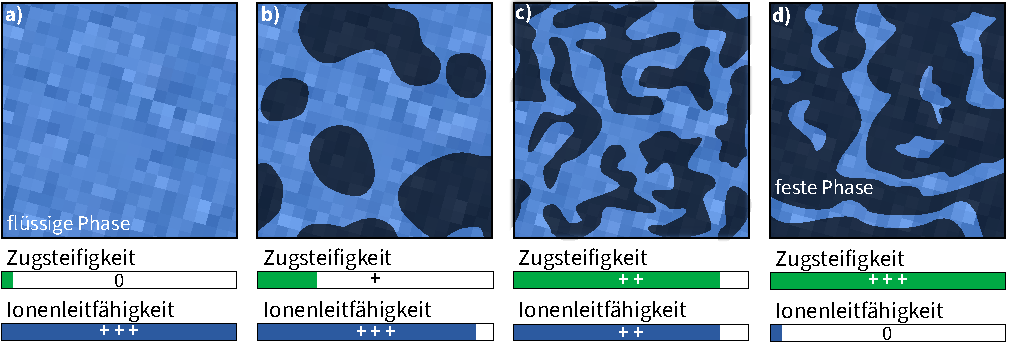
\includegraphics[width=\textwidth, angle=0]{bicontinous_electrolyte.pdf}
		\caption{\label{fig:bicontinous_electrolyte}Veränderung der Zugsteifigkeit und der Ionenleitfähigkeit mit zunehmenden festem Phasenanteil bei zweiphasigen Elektrolyten (a-d).}
\end{figure}
ZZweiphasige Elektrolyte bestehen aus einer festen Phase, die für die mechanischen Eigenschaften verantwortlich ist, und einer flüssigen oder gelförmigen Phase, die für die Leitung der Ionen zuständig ist~\cite{Ichino1995}. Durch die Einstellung des Phasenanteils und die Kontrolle der Porenarchitektur können die resultierenden Eigenschaften zwischen maximaler Leitfähigkeit und minimalen mechanischen Eigenschaften und umgekehrt eingestellt werden, siehe Bild~\ref{fig:bicontinous_electrolyte}. In simulativen Studien wurden mögliche ideale Architekturen und Phasenanteile zur maximalen Steigerung der Multifunktionalität bereits bestimmt~\cite{Lee2019,Tu2020}. Jedoch gibt es bisher nur eine bekannte Studie, die diese Nanostrukturen mithilfe von 3D-Druck fertigte~\cite{Zekoll2018}, die jedoch mit $2,7 \times 10^4$ $\si{\milli \siemens \per \cm}$ den angestrebten Grenzwert nicht überschreiten konnte. Der existierende Stand der Technik konzentriert sich daher hauptsächlich auf die Fertigung relativ ungeordneter Strukturen. Bei der Wahl des Phasenanteils sind dabei auch Untersuchungen aus der Perkolationstheorie, die sich mit der Bildung von weitreichenden Verbindungen in zufälligen Systemen beschäftigt, zu beachten. Untersuchungen mit zufällig angeordneten Kugeln zeigen, dass erst bei einem Anteil von 29,02~\% an leitender Phase ein Grenzwert überschritten wird, bei dem eine durchgehende Verbindung und damit die Möglichkeit des Ionentransports von einer Elektrode zur anderen sichergestellt werden kann~\cite{Li2020b}. Die gleiche Studie zeigt auch, dass durch Abweichung von der sphärischen Struktur dieser Anteil auf 22,94~\% reduziert werden kann. Die Perkolationstheorie ist somit ein wichtiges Mittel zur Untersuchung des Verhaltens von zweiphasigen Elektrolyten und bietet zum Beispiel Erklärungsansätze, warum bei bestimmten Anteilen von flüssiger Phase scheinbar plötzlich eine Steigerung der Ionenleitfähigkeit um mehrere Größenordnungen beobachtet wird~\cite{Melodia2023}.

Für die feste Phase haben sich auf Harz basierte Systeme hauptsächlich wegen ihrer einfacheren Löslichkeit und damit kleineren Porenbildung durchgesetzt. Jedoch treten vermehrt thermoplastische Systeme in den Vordergrund. Diese sind leichter in den Fertigungsprozess zu integrieren und bieten zusätzliche Sicherheit bei auftretenden Kurzschlüssen, da bei der entstehenden Wärmeentwicklung der Thermoplast schmilzt und die Poren verschließt, was einen weiteren Ladungsaustausch unterbindet.

Als Ausgangsmaterialien für die flüssige Phase kommen ionische Flüssigkeiten~\cite{Huang2022,Shirshova2013,Wendong2021,Shirshova2014,Dzienia2020}, Lithiumsalzlösungen in organischen Lösemitteln~\cite{Gienger2015,Sakakibara2017}, deren Kombination~\cite{Shirshova2014,Yu2016} und andere Systeme~\cite{Feng2017} in Betracht.

Feststoffelektrolyten bestehen meist aus einer Polymermatrix mit flexiblen Ketten, um die Bewegung eines gelösten Salzes zu ermöglichen. Der Hauptvorteil dieses Ansatzes liegt im Verzicht auf flüchtige oder brennbare Bestandteile und in den durch das Polymer bestimmten vergleichsweise guten mechanischen Eigenschaften. Allerdings ist die ionische Leitfähigkeit bei Raumtemperatur deutlich geringer als bei zweiphasigen Vertretern. Die Herstellung von Feststoffelektrolyten kann auf zwei Wegen erfolgen. Eine Möglichkeit stellt dabei die Polymerisation in Anwesenheit von Lithiumsalz dar. \textsc{Snyder et al.}~\cite{Snyder2007, Snyder2009} erreichten mit diesem Ansatz Ionenleitfähigkeiten von $1,6 \times 10^{-5}$ - $1,7 \times 10^{-3}$ $\si{\milli \siemens \per \cm}$ und damit verbundene Zugmodule von 552 bis 15~$\si{\MPa}$. Der zweite, häufig verwendete Ansatz nutzt eine Mischung von Polymeren mit Lithiumsalz. Für diese komplett festen zweiphasigen Elektrolytsysteme kommen häufig Epoxid~\cite{Matsumoto2011,Munoz2021,Wang2020b} oder PEO~\cite{Moreno2011,Ji2010,Guo2021} zum Einsatz.

\subsection{Separator}

Separatoren befinden sich zwischen den beiden Elektroden und dienen hauptsächlich dem Verhindern eines elektroschen Kurzschlusses. Daraus folgen die Anforderungen, dass Seperatormaterialien für Elektronen nicht durchlässig sind, aber für Ladungsträger Transportmechanismen bereitstellen~\cite{Kurzweil2015}. Um Kurzschluss auch bei mechansichen Belastungen zu verhindern werden werden außerdem Anforderungen an die mechansiche Belastbarkeit gestellt~\cite{Asp2015}. Weitere wichtige Eigenschaften sind eine hohe chemische und thermische Stabilität, insbesondere gegen Korrosion, geringe Dichte, geringe Dicke, große Verfügbarkeit und damit verbunden geringe Materialkosten~\cite{Beard2019}. Im Kontext von Strukturbatterien und der häufigen Verwendung von festen Elektrolytesystemen ist der Einsatz von Separatoren theoretische nicht notwendig, da anders als bei flüssigen Elektrolyen das Auseinanderhalten der Elektroden auch unter Druck gewährleistet werden kann. Jedoch ist im Rahmen von Sicherheitsbedenken und einer signifikanten Erschwerung des Herstellungsprozesses ohne diese der Einsatz von Seperatoren immer noch ein wichtiges Element in der Konzeptionierung von Strukturbatterien~\cite{Asp2015, Hubert2022}.
Das meisten verwendete Separatormaterial ist Glasfaser~\cite{Zhou2022}. Jedoch exitieren auch vielversprechende Kandidaten, wie Polymerbasierte Separatoren, Keramiken und Cellulose~\cite{Simon2008, Greenhalgh2023}, siehe Tabelle~\ref{tab:separator_comp}
\begin{table}[h!]
    \caption{Properties of different types of separators}
    \label{tab_separator_comp}
    %\begin{adjustwidth}{-\extralength}{0cm}
    \newcolumntype{C}[1]{>{\hsize=#1\hsize\centering\arraybackslash}X}%
    \begin{tabularx}{\textwidth}{
    %C{0.6}
    C{1} 
    C{1.8} 
    C{0.8} 
    C{0.8} 
    C{0.8} 
    C{0.6}
    }
        \toprule
        \textbf{Separatortyp}
        &\textbf{Separatormaterial} 
        &\textbf{Ionische Leit- fähigkeit\textsuperscript{*} (mS/cm)} 
        &\textbf{Zug- steifigkeit\textsuperscript{*} (GPa)}
        & \textbf{Festigkeit\textsuperscript{*} (MPa)}
        &\textbf{Ref.} \\
        \midrule
        %\legendsep{c0}&
        Glassfaser&Glassfaser&1.13&21
        &325
        &\cite{Deka2017}\\
        %\midrule
        \addlinespace
        %\legendsep{c10}&
        Polymer&RF/PLA&110&0.3271
        &15.2
        &\cite{Vargun2020}\\
        %\midrule
        \addlinespace
        %Gel polymer electrolyte&$\mathrm{PVA/KOH/K_3[Fe(CN)_6]}$&45.56&n.a.&n.a.&\cite{maHighPerformanceSolidstate2014}\\
        %%\midrule
        %\legendsep{c4}&
        Feststoff- elektrolyt&$\mathrm{PEGDGE/TETA/EMIBF_4}$&0.2&26
        &350
        &\cite{Hubert2022, Choi2022}\\
        %\midrule
        \addlinespace
        %\multirowcell{2}{\legendsep{c6}}&
        \multirowcell{2}{Keramik}
            &$\mathrm{PVDF/PPG/LiCl/CaTiO_3}$&n.a.&1.2
            &65
            &\cite{Alvarez‐Sanchez2019}\\
            &$\mathrm{PVB/Al_2O_3NW}$&13.5&n.a.
            &30
            &\cite{Liu2020a}\\
        %\midrule
        \addlinespace
        %Diode-like polymer electrolyte&PVP/PEI/SWCNT&n.a.&n.a.&n.a.&\cite{chowdhurySupercapacitorsElectricalGates2019}\\
        %%\midrule
        %Ceramic&NPs/PTFE/SiC&n.a.&n.a.&1.3&\cite{qinCeramicBasedSeparatorHighTemperature2018,zhaoInorganicCeramicFiber2017}\\
        %%\midrule
        %Tree-leave&Quercus rubra&n.a.&n.a.&n.a.&\cite{chenTrashTreasureFallen2022,wangMechanicalCharacteristicsTypical2010}\\
        %%\midrule
        %Eggshell membrane&Eggshell membrane&3.8&n.a.&6.59&\cite{yuUsingEggshellMembrane2012}\\
        %%\midrule
        %\legendsep{c8}&
        Cellulose&MCC/AMIM-Cl&298.6&5.43
        &71.71
        &\cite{Ahankari2022, Xu2020}\\
        %%\midrule
        %Graphene oxide&Graphene oxide paper&n.a.&n.a.&n.a.&\cite{shulgaSupercapacitorsGrapheneOxide2015,comptonTuningMechanicalProperties2012}\\
        %%\midrule
        %Metal-organic framework&Metal-organic framework&n.a.&n.a.&n.a.&\cite{mengMetalOrganicFrameworks2015,bundschuhMechanicalPropertiesMetalorganic2012}\\
        \bottomrule
    \end{tabularx}
    %\end{adjustwidth}
    \noindent{\footnotesize{\textsuperscript{*} The abbreviation not available (n.a.) is used.}}
\end{table}

Glasfaserseparatoren finden großen Einsatz wegen ihrer hohen mechanischen Belastbarkeit, ihrer sehr hohen thermischen und elektrochemischen Stabilät und relativ geringen Materialkosten~\cite{Luo2015,Asp2019,Asp2021,Liu2022}. Allerdings haben sie im Vergleich zu anderen Materialkandiadten eine signifikant höhere Dicke und benötigen eine hohe Maschenweite um einen hohen Ionenaustausch zu ermöglichen, siehe Bild~\ref{fig:separator_transportation}, was allerdings mit einem höheren Kurzschlussrisiko einher geht~\cite{Danzi2021,Zhou2022}. 
Im Kontext von faserbasierten Separatoren wurden außer Glasfasern auch Aramidfaser eingehen betrachtet~\cite{Jin2023}. Hervorzuheben ist hierbei ihre Fähigkeit Dendritwachstum zu verhindern und zeigt bei Lithiumionenbatterien oft ein besser Zyklenverhalten gegenüber Glasfasern~\cite{Tung2015,Wang2021a}.
\begin{figure}[h]
	%\raggedleft
		%\def\svgwidth{\columnwidth}
        \center
	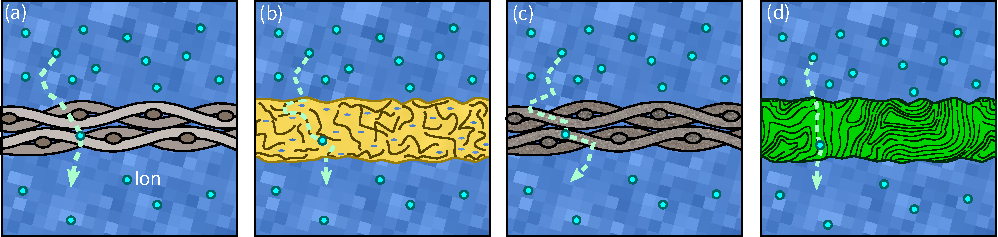
\includegraphics[width=\textwidth, angle=0]{separator_transportation.pdf}
		\caption{\label{fig:separator_transportation}Visualisierung verschiedener Separatormaterialien und der jeweligen Ionentransportwege (gestrichelte Linie) für: (a) Gewebe, (b) Polymer-, (c) Keramikseparator und (d) Cellulose~\cite{Zschiebsch2024}.}
\end{figure}


Polymerseparator

Keramische Seperatormaterialien zeichnen sich besonders durch ihre hohe thermische Stabilität aus. 

Das Interesse an Cellulose ist in den letzten Jahren zusammen mit einem wachsenden Forschungsfeld zu den Themenfeldern ''nachwachsende Rohstoffe'' und ''recyclebare elektrische Speicher'' immer mehr gewachsen~\cite{Liang2018,Teng2020}. Cellulose zeigt dabei eine sehr hohe Ionenleitfähigkeit, und eine gute, wenn auch im Vergleich mit Glasfasern deutlich geringer, mechanische Festigkeit und Zugsteifigkeit~\cite{Xu2020}, siehe Tabelle~\ref{tab:separator_comp}. Eine Möglichkeit der Steigerung der Steifigkeit stellt dabei dei Verwendung von Nanocellulose dar die Zugsteifigkeiten von bis zu 130~$\si{\GPa}$ erreicht~\cite{Dufresne2013,Zhang2019}.

\subsection{Pouchfolie}
Herkömmliche Pouchzellen sind mit einer kunststoffbeschichteten Aluminiumhülle vor Umwelteinflüssen geschützt. Insbesondere verhindert diese, dass Feuchtigkeit in die Batterie eindringt und giftige oder brennbare Stoffe aus der Batterie entweichen können. Außerdem ermöglichen die guten mechanischen und Wärmeleiteigenschaften der Aluminiumfolie eine geringe Gesamtmasse und eine effizientere Temperaturregulierung der Zellen. Eine zunehmend wichtiger werdende Aufgabe, die allerdings noch nicht hinreichend erfüllt wird, ist das Aufbringen eines äußeren Zelldrucks.

In mehreren Studien konnte gezeigt werden, dass durch einen hohen externen Druck die Kontaktierung zwischen Elektrode und Elektrolyt verbessert wird, was einen besseren Ionen- und Elektronentransport bewirkt. Außerdem können unerwünschte Nebenreaktionen unterdrückt werden, wie etwa Gasbildung und Dendritwachstum, was den Lithiumverlust beim Laden und Entladen reduziert und somit dem Kapazitätsverlust entgegenwirkt und das Batterieleben verlängert \cite{Mussa2018,Mueller2019,Sakamoto2019}. Besonders Batterien mit Feststoffelektrolyten benötigen einen deutlich höheren Druck, um den Kontakt zwischen Elektrode und Elektrolyt zu gewährleisten \cite{Boaretto2021}. Jedoch existiert zurzeit noch keine zufriedenstellende Lösung. Zwar wird bereits bei der Herstellung mittels Verpressen der Elektroden ein gewisser Druck realisiert, allerdings können größere Drücke damit nicht appliziert oder über längere Zeit aufrechterhalten werden \cite{Garayt2023}. Daher wird oft versucht, durch eine externe Einspannung auf Systemebene diesen Druck aufzubringen. Jedoch entsteht durch die innere Reibung der Batterien kein gleichmäßiger Druckverlauf, was dazu führt, dass äußere Zellen stärker belastet werden und weiter innen liegende Zellen kaum von dem äußeren Druck profitieren. Auch haben höhere Ausgleichsdrücke das Problem, dass diese eine höhere Anstrengung für das Gesamtpaket darstellen, was zu dickeren Materialien und damit einer niedrigeren Gesamtenergiedichte führt.

Einzig die Knopfzellen, die durch eine integrierte Feder einen definierten Druck auf eine im Verhältnis zur Pouchzelle deutlich kleinere Fläche ausüben, sind die einzige bekannte Lösung zu diesem Problem. Hinzukommt, dass auch hier der Massenanteil von Gehäuse zu Zelle deutlich höher ist als bei Pouchzellen.

Für Strukturbatterien sind bisher keine Alternativen zur herkömmlichen Aluminiumpouchfolie untersucht worden \cite{Ye2024}. Jedoch gibt es viele Gruppen, die ihre Strukturbatterien mit Pouchfolie zusätzlich in einen kohlefaserverstärkten Kunststoff einbetten \cite{Pattarakunnan2020,Asp2021}.

\section{Aktuelle Ansätze zur Entwicklung und Auslegung von Strukturbatterien}

\section{Ungelöste Herausforderungen in der Entwicklung von Strukturbatterien}
Erstellung Bild siehe Kommentar in .tex Datei
%Bild in Inkscape erzeugt und als SVG sowie pdf_tex speichern (Speichern unter -> .pdf -> Text in PDF weglassen und LaTex Datei erstellen). 


\begin{figure}[h]
	%\raggedleft
		%\def\svgwidth{\columnwidth}
	\def\svgscale{0.98}
		\input{testbild.pdf_tex} 
		\caption{\label{fig:testbild}Testbild erzeugt mit Inkscape}
\end{figure}

Bild \ref{fig:testbild} %\cite{Dannemann.Kucher_et.al_AppliedSciences_2018}  

Verwendung Package SIUNITX %(siehe Datei latex_package_readme_siunitx.pdf)   

Anzugsdrehmoment von $M_{\textnormal{a}}=\SI{1.1}{\newtonmetre}$

von \SI{1}{\kilo\hertz} bis \SI{15}{\kilo\hertz}

mittlere Temperaturänderung von $\left\langle \Delta T_{\textnormal{p}}\right\rangle(t)<\SI{0.5}{\degreeCelsius}$

Masse von $m_{\textnormal{p}}=\SI[separate-uncertainty]{0.884 (15)}{\gram}$

(siehe Abschnitt \ref{ch:anhang})
\chapter{\label{sec:modelling_SB}Modellierung von Strukturbatterien}
Die Modellierung von Strukturbatterien auf der Mirkoskalenebene wurde in den letzten Jahren maßgeblich durch die Arbeiten von Carlstedt~\cite{Carlstedt2018,Carlstedt2019,Carlstedt2022a,Carlstedt2023} vorrangetrieben. Modelle und die Kopplung der mechansichen, elektrochemischen und thermischen Effekte wurde bereits erbracht~\cite{Carlstedt2022,Carlstedt2022b}. Des Weiteren sind aus der Forschung zu herkömmlichen Batterien auch noch andere Ansätze bekannt, die in Kaptiel~\ref{sec:existing_micro_models} kurz erläutert werden sollen. Die Modelle von Carlstedt beschreiben, allerdings vorranging das Verhalten auf der Mikro- oder Partikelebene. Jedoch existiert eine Vielzahl an Arbeiten, die gezeigt haben, wie für konventionelle Batterien eine mittels Homogenisierung, diese Modelle für höhere Skalen adaptiert werden können. Mit Hilfe dieser Methoden wird in Kapitel~\ref{sec:homogenisation} die Modellierung für die Makroebene hergeleitet.

\section{\label{sec:existing_micro_models}Bestehende Mikroskalen Modellierungen}

Die auf der Mirko- oder Partikelebene stattfindenden Prozesse sind unabhängig davon, ob eine konventionelle oder eine Strukturbatterie modelliert wird. Einige Prozesse spielen allerdings für konventionelle Batterien nur eine untergeordente Rolle, weshalb diese oft ignoriert oder vereinfacht werden~\cite{Carlstedt2020a}. Der Ionentransport ist dabei der wichtigste Prozess~\cite{Carlstedt2019b}. Dabei bestehen nach \textsc{Newman} wesentliche Unterschide zwischen flüssige und festen Phasen~\cite{Newman2021}. Da sowohl  konventionelle Batterien, als auch Strukturbatterien, mit zweiphasigen Elektrolyten einen Ionentransport durch beide Phasen besitz lassen sich kann ihr Verhalten in erster Näherung durch die folgenden fünf Differnetialgleichungen\footnote{auch unter dem Namen \textsc{Doyle}-\textsc{Fuller}-\textsc{Newman}-Modell bekannt} beschrieben werden~\cite{Plett2015}.
\begin{enumerate}
    \item Ladungserhalt in homogenen Festkörpern
    \begin{equation}
        \nabla \cdot \boldsymbol{i}_{\text{s}} = \nabla \cdot \left( - \sigma \cdot \nabla \phi_{\text{s}} \right) = 0
    \end{equation}

    \item Massenserhalt in homogenen Festkörpern
    \begin{equation}
        \frac{\partial c_{\text{s}}}{\partial t}  = \nabla \cdot \left( D_{\text{s}} \nabla c_{\text{s}} \right) = 0
    \end{equation}

    \item Massenerhalt in dem homogenen Elektrolyt
    \begin{equation}
        \frac{\partial c_e}{\partial t} = \nabla \cdot \left( D_e   \nabla c_e \right) - \frac{\boldsymbol{i}_{\text{e}} \cdot    \nabla t_+^0}{F_{\text{K}}} - \nabla \cdot \left( c_{\text{e}} \boldsymbol{v}_0\right)
    \end{equation}

    \item Ladungserhalt  in dem homogenen Elektrolyt
    \begin{equation}
        \nabla \cdot \boldsymbol{i}_{\text{e}} = \nabla \cdot \left(    - \kappa \nabla \phi_{\text{e}}  -\frac{2\kappa R_{\text{K}} T}{F_{\text{K}}} \left(  1+ \frac{\partial \ln f_\pm}{\partial \ln c_{\text{e}}}\right)   \left( t_+^0-1\right) \nabla \ln c_{\text{e}} \right) = 0
    \end{equation}

    \item Ionentrasport zwischen fester und flüssiger Phase
    \begin{align}
        j &= \frac{i_0}{F}\left( \exp \left(\frac{\left(1-\alpha\right)  F}{RT}\eta \right) - \exp \left(-\frac{\alpha F_{\text{K}}}{R_{\text{K}} T}  \eta\right) \right)\\
        i_0 &= n F_{\text{K}} k_0 \left(\prod_i c_{o,i}\right)^{1-\alpha} \left( \prod_i c_{r,i}\right)^\alpha\\
        \eta &= (\phi_{\text{s}}-\phi_{\text{e}}) - U_{\text{ocp}}
    \end{align}
\end{enumerate}
Dabei beschreibt $\boldsymbol{i}$ die Ladungsdichte, $\sigma$ die materialabhängige  Leitfähigkeit, $\phi$ das elektrische Potenzial, $c$ die Ladungsträgerkonzentration, $D$ der materialabhängige Diffusionskoeffizient, $\boldsymbol{t}^0_+$ die Hittorfsche Überführungszahl der Kationen im bezug auf das Elektrolytsystem, $F_{\text{K}}$ Farrady-Konstante, $\boldsymbol{v}_0$ die Geschwindigkeit des Elektrolytes, $\kappa$ die ionische Leitfähigkeit, $R_{\text{K}}$ die ideale Gaskonstante, $T$ die Temperatur, $f_{\pm}$ der mittlere molare Aktivitäntskoeffizient, $j$ die molare Ionenflussdichte, $i_0$ die Austauschladungsdichte\footnote{Vereinfacht sich für Lithium und Natrium zu: $i_0 = F_{\text{K}} k_0 c_e^{1-\alpha} (c_{s,max}-c_{s,e})^{1-\alpha} c_{s,e}^\alpha$},  $\eta$ das Reaktionsüberpotenzial, $k_{0,K}$ effektive Rekationsratenkonstante, $U_{\text{ocp}}$ das Leerlaufspannung und asymetrischer Ladungungstransferkoeffizient $0<\alpha<1$ definiert durch
\begin{equation}
        \alpha = \left|\frac{\Delta E_{\text{a,red}}}{\Delta G_0}\right|
\end{equation}
das Verhältnis aus Änderung der Aktivierungsenergie der Reduktionsmittel ($\Delta E_{\text{a,red}}$) und Änderung der Gibbs-Energy der Oxidationsmittel ($\Delta G_0$).

Neben dem Ladungstransport spielen Temperaturentwicklung und die Entstehung mechansicher Spannungen eine Rolle.
Dabei hängt die Temperaturentwicklung in der festen und flüssigen Phase von $\rho$ der Dichte, $c_\text{P}$ der spezifischen Wärmekapazität, $\lambda$ der Wärmeleitfähigkeit und dem elektrischen Strom ab.
\begin{align}
    \rho_{\text{s}} c_{\text{P,s}} \frac{T_{\text{s}}}{\partial t} &= \nabla \cdot (\lambda_{\text{s}} \nabla T_{\text{s}}) - \boldsymbol{i}_{\text{s}} \cdot \nabla \phi_{\text{s}}\\
    \rho_{\text{e}} c_{\text{P,e}} \frac{T_{\text{e}}}{\partial t} &= \nabla \cdot (\lambda_{\text{e}} \nabla T_{\text{e}}) - \boldsymbol{i}_{\text{e}} \cdot \nabla \phi_{\text{e}}
\end{align}

Mechanische Spannung hat besonders im Kontext von Strukturbatterien eine signifikante Bedeutung~\cite{Carlstedt2020b}, wird aber auch bei konventionellen Batterien als entscheidenter Faktor für einige Alterungsmechanismen berücksichtigt~\cite{Mueller2019}. Die mechanische Spannung kann dabei nur in der festen Phase auftreten.
\begin{equation}
    -\nabla \cdot \boldsymbol{\sigma} = \boldsymbol{0}
\end{equation}
Durch \textsc{Hook} lässt sich außerdem die mechanische Spannugn mit der Dehnung als lineare Abhängigkeit darstellen.
\begin{equation}
    \boldsymbol{\sigma} = \boldsymbol{C} \boldsymbol{\varepsilon}_{mech}
\end{equation}
Bei dem Elastizitätstensor $\boldsymbol{C}$ wird im Kontext von Strukturbatterien je nach Material zwischen einer isotrop\footnote{z.B. Metallelelektrode, Aktivmaterial, Polymerphase}, transversal-isotropen\footnote{z.B. einzelne Kohlenstofffaser} und orthotropen\footnote{z.B. Kohlenstofffasergewebe, Glasfaserseparator} Beschreibung unterschieden.
\begin{align}
\boldsymbol{C}^{-1}_{\text{iso}} &= 
\begin{bmatrix}
    \frac{1}{E} & -\frac{\nu}{E} & -\frac{\nu}{E} & 0 & 0 & 0 \\
    -\frac{\nu}{E}& \frac{1}{E} & -\frac{\nu}{E} & 0 & 0 & 0 \\
    -\frac{\nu}{E} & -\frac{\nu}{E} & \frac{1}{E} & 0 & 0 & 0 \\
    0 & 0 & 0 & \frac{2(1+\nu)}{E} & 0 & 0 \\
    0 & 0 & 0 & 0 & \frac{2(1+\nu)}{E} & 0 \\
    0 & 0 & 0 & 0 & 0 & \frac{2(1+\nu)}{E} \\
\end{bmatrix}\\
\boldsymbol{C}^{-1}_{\text{trans}} &= 
\begin{bmatrix}
    \frac{1}{E_{1}} & -\frac{\nu_{12}}{E_{1}} & -\frac{\nu_{13}}{E_{1}} & 0 & 0 & 0 \\
    -\frac{\nu_{12}}{E_{1}}& \frac{1}{E_{2}} & -\frac{\nu_{23}}{E_{2}} & 0 & 0 & 0 \\
    -\frac{\nu_{13}}{E_{1}} & -\frac{\nu_{23}}{E_{2}} & \frac{1}{E_{2}} & 0 & 0 & 0 \\
    0 & 0 & 0 & \frac{2(1+\nu_{23})}{E_{2}} & 0 & 0 \\
    0 & 0 & 0 & 0 & \frac{1}{G_{31}} & 0 \\
    0 & 0 & 0 & 0 & 0 & \frac{1}{G_{12}} \\
\end{bmatrix}\\
\boldsymbol{C}^{-1}_{\text{ortho}} &= 
\begin{bmatrix}
    \frac{1}{E_{1}} & -\frac{\nu_{12}}{E_{1}} & -\frac{\nu_{13}}{E_{1}} & 0 & 0 & 0 \\
    -\frac{\nu_{12}}{E_{1}}& \frac{1}{E_{2}} & -\frac{\nu_{23}}{E_{2}} & 0 & 0 & 0 \\
    -\frac{\nu_{13}}{E_{1}} & -\frac{\nu_{23}}{E_{2}} & \frac{1}{E_{3}} & 0 & 0 & 0 \\
    0 & 0 & 0 & \frac{1}{G_{23}} & 0 & 0 \\
    0 & 0 & 0 & 0 & \frac{1}{G_{31}} & 0 \\
    0 & 0 & 0 & 0 & 0 & \frac{1}{G_{12}} \\
\end{bmatrix}
\end{align}

\begin{figure}[!ht]
	%\raggedleft
		%\def\svgwidth{\columnwidth}
        \center
		\includegraphics[width=0.99\textwidth, angle=0]{carlstedt.pdf}
		\caption{\label{fig:carlstedt}a) Schematische Darstellung der zu analysierenden Kohlenstofffaser-Strukturbatterie und LFP Zelle angelehnt an Studien von \textsc{Carlstedt}~\cite{Carlstedt2022b}. b) 2D-Model für die FEM Berechnung. c) Der Angelegte Strom als treibende Randbedingung über die Zeit. e) Die elektrische Spannung und Stromdichte über die Zeit und die Lithiumkonzentration an den beiden Zeitpunkten $t_1= 2000s$ und $t_2= 6000s$. f) Die gemittelte Temperatur in der Halbzelle über die Zeit und die Temperaturverteilung bei $t_1$ und $t_2$. g) Die mechansichen Spannungskomponenten $\sigma_{11}$ und $\sigma_{22}$ zu $t_1$ und $t_2$.}
\end{figure}

Besonders bei den Materialien, die als Interkalationsort dienen, haben Untersuchungen von \textsc{Duan}~\cite{Duan2021} gezeigt, dass die Elastizitätsmodule näherungsweise linear von der Ionenkonzentration abhängig sind.
\begin{equation}
    E(c_{s}) = E_0 + \frac{c_{s}}{c_{s,1}} (E_1 - E_0)
\end{equation}

Die Gesamtdehnung $\boldsymbol{\varepsilon}$ ergibt sich dabei aus Summe der elektrochemischen, thermischen und mechanischen Einflüsse
\begin{equation}
    \boldsymbol{\varepsilon} = \boldsymbol{\varepsilon}_{echem} +\boldsymbol{\varepsilon}_{th} + \boldsymbol{\varepsilon}_{mech}
\end{equation}
und wird direkt aus dem Verschiebungsfeld $u$ bestimmt werden.
\begin{equation}
    \boldsymbol{\varepsilon} = \frac{1}{2}\left[\left(\nabla u\right)^T + \left(\nabla u\right)\right]
\end{equation}
Die themische und elektrochemischen Dehnungsanteile hängen dabei durch den jeweiligen Ausdehnungskoeffizeinten $\boldsymbol{\alpha}$ linear von der Veränderung der Temperatur bzw. Konzentration ab.
\begin{align}
    \boldsymbol{\varepsilon}_{echem} &= \boldsymbol{\alpha}_{echem} \left(c_{\pm}-c_{\pm,0}\right)\\
    \boldsymbol{\varepsilon}_{th}  &= \boldsymbol{\alpha}_{th}\left( T - T_0\right)
\end{align}

Die aus den Gleichungen folgende mikroskalige Simulation kann benutzt werden um Zellen mit Geometrien in ähnlichen Größenskalen zu simulieren~\cite{Plett2015}. Angelehnt an Arbeiten von \textsc{Carlstedt}~\cite{Carlstedt2022b}\footnote{Die Materialwerte und Geometrie, sowie die Randbedingung wurden aus der Arbeit entnommen um einen Vergleich zu haben.} wird dies für eine Kohlenstofffaser-LFP-Zelle gemacht (Bild~\ref{fig:carlstedt}). Die Zelle durch läuft dabei einen Entladungs- und Ladezyklus innerhalb von 2,2 h. Die Simulationszeit betrug dabei 34,6 h auf einem Berechnungsserver der HTWK\footnote{Unter voller Ausnutzung von zwei eingebauten CPUs der Marke AMD EPYC 75F3 mit einer Taktrate von 2,95 Ghz und jeweils 32 Kernen}. Der hohe Berechnungsaufwand für breits einen Ladezykls macht diesen Anasatz jedoch ungeeignet um eine Vielzahl an Varianten und größere, mehrzellige Batteriesysteme vorauszulegen.




\section{\label{sec:homogenisation}Überführung der Mikroskaligen Modellierungsansätze in makroskalige Modelle durch Homogenisierung}

Die Modellierung der einzelnen phyiskalischen Prozesse sind oft einfacher auf der Mikroskale zu beschreiben~\cite{Plett2015}. Mit Hilfe dieser lassen sich Geometrie-, Verteilungs- und Clusterbildungseinflüsse ermitteln~\cite{Newman2021}. Jedoch ist der mit der hohen Komplexität durch die verschiedenen Skalenbereiche verbunde Berechnungsaufwand zu groß um mehrere Zellen damit zu simulieren~\cite{Liu2019}. Daher werden makroskalige Modelle benötigt, die den Berechnungsaufwand durch Homogenisierung und Modellvereinfachunngen reduziern~\cite{Plett2015}.

Ein häufig verwendeter Ansatz stellt dabei die Mittelung der physikalischen Eigenschaften über ein repräsentatives Volumenelement dar~\cite{Burow2016,Arunachalam2019,Li2020}. Die dazu mathematischen Grundlagen basieren auf drei Volumenmittlungstheoremen~\cite{Gray1977}.
\begin{enumerate}
    \item Volumenmittlung für ein skalares Feld $\psi$ 
    \begin{equation}
        \varepsilon_{\alpha} \overline{\nabla \psi_{\alpha}} = \nabla \left(\epsilon_{\alpha} \bar{\psi}_{\alpha} \right) + \frac{1}{V} \iint_{A_{\alpha \beta(\boldsymbol{x},t)}}\psi_{\alpha} \hat{\boldsymbol{n}}_{\alpha} \text{d}A
    \end{equation}
    \item Volumenmittlung für ein Vektorfeld $\boldsymbol{\psi}$
    \begin{equation}
        \varepsilon_{\alpha} \overline{\nabla \cdot \boldsymbol{\psi}_{\alpha}} = \nabla \cdot \left(\epsilon_{\alpha} \bar{\boldsymbol{\psi}}_{\alpha} \right) + \frac{1}{V} \iint_{A_{\alpha \beta(\boldsymbol{x},t)}}\boldsymbol{\psi}_{\alpha} \cdot \hat{\boldsymbol{n}}_{\alpha} \text{d}A
    \end{equation}
    \item Volumenmittlung für die zeitliche Änderung eines skalaren Feldes $\psi$ 
    \begin{equation}
        \varepsilon_{\alpha} \overline{\left[\frac{\partial \psi_{\alpha}}{\partial t}\right]} = \frac{\partial \left(\epsilon_{\alpha} \bar{\psi}_{\alpha} \right)}{\partial t} - \frac{1}{V} \iint_{A_{\alpha \beta(\boldsymbol{x},t)}}\psi_{\alpha} \boldsymbol{v}_{\alpha \beta} \cdot \hat{\boldsymbol{n}}_{\alpha} \text{d}A
    \end{equation}
\end{enumerate}
Dabei beschreibt $\bar{\psi}_{\alpha}$ bzw. $\bar{\boldsymbol{\psi}}_{\alpha}$ die intrinsischen Mittelung über Phase $\alpha$. Diese Art der Mittelung wird nur über das von Phase $\alpha$ eingenommene Volumen\footnote{Hier als zwei Phasensystem mit der zweiten Phase $\beta$ betrachtet.} ermittelt. Die intrinische Mittelung erlaubt gegenüber einer klassischen Mittelung $\langle \psi_{\alpha} \rangle$, welcher auf das Volumen des gesamten Gebietes bezogen ist, eine größere Flexibilität und wieder Verwendbarkeit. Mittels des Volumenanteils $\epsilon_{\alpha}$
\begin{equation}
    \varepsilon_{\alpha} = \frac{V_{\alpha}(\boldsymbol{x},t)}{V} 
\end{equation}
können die beiden Mittelungsarten in einander umgewandelt werden.
\begin{equation}
    \langle \psi_{\alpha} \rangle = \varepsilon_{\alpha} \bar{\psi}_{\alpha}
\end{equation}

Mit Hilfe der drei Volumenmittelungstheoreme lassen sich die folgenden vier Gleichungen herleiten~\cite{Doyle1995}.
\begin{enumerate}
    \item Volumengemittelte Annäherung des Ladungserhaltes in der festen Phase der porösen Elektrode
    \begin{equation}
        \nabla \cdot \left(\sigma_{\text{eff}} \nabla \hat{\phi}_{s} \right) = a_s F_{\text{K}} \hat{j}
    \end{equation}
    \item Volumengemittelte Annäherung des Ladungserhaltes in der Elektrolytphase der porösen Elektrode
    \begin{equation}
        \nabla \cdot \left(\kappa_{\text{eff}} \nabla \hat{\phi}_e + \kappa_{D, \text{eff}} \nabla ln \hat{c}_e\right) + a_s F_{\text{K}} \hat{j} = 0
    \end{equation}
    \item Volumengemittelte Annäherung des Massenerhaltes in der Elektrolytphase der porösen Elektrode
    \begin{equation}
        \frac{\partial \left(\epsilon_e \hat{c}_e \right)}{\partial t} = \nabla \cdot \left(D_{e,\text{eff}}\nabla\hat{c}_e\right) + a_s (1+t^0_+) \hat{j}
    \end{equation}
    \item Volumengemittelte Annäherung der mikroskopischen Butler-Volmer Beziehung für den Ionenphasenwechsel
    \begin{equation}
        \hat{j} = j(c_{s,e},\hat{c}_e,\hat{\phi}_s,\hat{\phi}_e)
    \end{equation}
\end{enumerate}

Analog lassen sich für die Temparatur und die Spannung die folgenden Zusammenhänge aufstellen.
\begin{enumerate}
    \item Spezialfall Massenserhalt in kugelförmigen Festkörpern
    \begin{equation}
        \rho_{\text{eff}} c_{\text{P,eff}} \frac{T_{\text{eff}}}{\partial t} = \nabla \cdot (\lambda_{\text{eff}} \nabla T_{\text{eff}}) - \boldsymbol{i}_{\text{eff}} \cdot \nabla \phi_{\text{s}}
    \end{equation}
    \item Homogenisierung der Steifigkeit
    \begin{equation}
    \boldsymbol{\sigma} = \boldsymbol{C}_{\text{eff}} \boldsymbol{\varepsilon}_{\text{mech}} 
    \end{equation}
\end{enumerate}

Für die Massenerhaltung in der festen Phase\footnote{Die Materialien, die als Interkalationsort dienen} ist eine Volumenmittelung wegen der Butler-Volmer Randbedingung nicht möglich~\cite{Plett2015}.Allerdings können durch Geometrievereinfachungen Freiheitsgrade reduziert werden und zusätzlicher Berechnungsaufwand vermieden werden. Im Kontext von Strukturbatterien ist der an der Interkalation aktiv teilnehmende Teil Partikel- oder Faserförmig, welche durch Kugeln oder Zylinder approximiert werden könnent~\cite{Newman2021}.
\begin{enumerate}
    \item Spezialfall Massenserhalt in kugelförmigen Festkörpern
    \begin{equation}
    \frac{\partial c_{\text{s}}}{\partial t} = \frac{1}{r^2} \frac{\partial}{ \partial r} \left[ D_{\text{s}} r^2 \frac{\partial c_{\text{s}}}{\partial r}\right]
    \end{equation}
    \item Spezialfall Massenserhalt in zylindrischen Festkörpern
    \begin{equation}
    \frac{\partial c_{\text{s}}^{\pm}}{\partial t} = \frac{1}{r} \frac{\partial}{ \partial r} \left[ D_{\text{s}} r \frac{\partial c_{\text{s}}}{\partial r}\right] + \frac{\partial}{ \partial z}\left[D_{\text{s}}  \frac{\partial c_{\text{s}}}{\partial z}\right]
    \end{equation}
\end{enumerate}
Die Randbedingung
\begin{align}
    \frac{\partial c_{\text{s}}^{\pm}}{\partial r}(x,0,t) &= 0 \\
    \frac{\partial c_{\text{s}}^{\pm}}{\partial r}(x,R_{\text{p,s}}^{\pm},t) &= -\frac{1}{ D_{\text{s}}^\pm} j_{n}^{\pm}(x,t)
\end{align}
und
\begin{equation}
j_{n}^{\pm}(t) = \mp \frac{I(t)}{F a^{\pm} L^{\pm}}
\end{equation}

Durch ermittlung effektiver physikalischer Eigenschaften werden dabei die Inhomognitäten auf der Mikroskale durch ein Kontinuum auf der Markoskale beschrieben~\cite{Plett2024}. Die Genauigkeit dieses Ansatz hängt jedoch stark von dem zu betrachten Dimensionen ab~\cite{Plett2015}. Durch die Beschreibung als Kontinuum können Einglüsse wie etwa eine lokal höhere Porendichte nur aufwendig berücksichtigt werden~\cite{Mei2019}. Bei der Analyse von deutlich größeren Skalen, als die Inhomogenität, zeigen diese Modelle dafür eine hohe Genauigkeit~\cite{Plett2015}. 



\begin{figure}[!h]
	%\raggedleft
		%\def\svgwidth{\columnwidth}
        \center
		\includegraphics[width=\textwidth, angle=0]{simulation_model.pdf}
		\caption{\label{fig:homogenisation}Mehrskalige Homogenisierung der Strukturbatterie durch Abstraktion der Geometrie, }
\end{figure}

\begin{figure}[!h]
	%\raggedleft
		%\def\svgwidth{\columnwidth}
        \center
		\includegraphics[width=0.75\textwidth, angle=0]{bending.pdf}
		\caption{\label{fig:bending}Validierung des 3-Punkt-Biegefalls durch: a) Visueller Vergleich von Simulation und Experiment und b) Kraftverlauf in Abhängigkeit der Durchbiegung für Pouchzellen mit und ohne Elektrolyt.}
\end{figure}



\chapter{Entwicklung einer hybriden Auslegung von Strukturbatterien}
Die Modelle, die sich aus den Arbeiten von \textsc{Carlstedt}, \textsc{Doyle}, \textsc{Newman}, \textsc{Fuller} und \textsc{Plett} ergeben sind mit einem hohen hohen Detailgrad versehen. Dieser Detailgrad erlaubt eine hohe physikalische Präzesion, jedoch sorgt dies gleichzeitig für eine hohe Anzahl an Parametern, die aufwenig bestimmt werden müssen. Damit entsteht das Problem, dass in bestimmten Konstellationen es schneller und günstiger ist direkt Experimente mit allen Materialkombinationen zu machen, als erst alle benötigten Material- und Interaktionsparamter zu bestimmen. Um dies einzuschätzen und eine möglichst optimale Entwicklungsstrategie wird in Kapitel~\ref{sec:efficent_development} ein entsprechendes Auswahl und Bewertungsrahmenwerk entwickelt. Mit Hilfe dieses werden in den Kapiteln~\ref{sec:improve_elchem} und \ref{sec:improve_mech} eine Reihe an häufig gültigen Vereinfachungen der elektrochemische und mechansichen Modellierung unternommen. Um die Einsatzfähigkeiten der verschiedenen Strukturbatterie automatisiert bewerten zu können wird in Kaptiel~\ref{sec:automated_failure} ein Versagens- und Risikoabschätzung vorgestellt. Abschließend wird in Kapitel~\ref{sec:digitalisation} auf die Umsetzung der digitalen und automatisierten Vorauswahl geegineter Strukturbatteriekonfigurationen eingegangen.

\section{\label{sec:efficent_development}Konzeptionierung eines effizienten Entwicklung von Strukturbatterien}
Für den effektiven Einsatz der Modellen für die Vorhersage von mechansichen und elektroschmeischen Eigenschaften wurde eine Vielzahl an Anforderungen an die Modellierung gesammelt:
\begin{itemize}
    \item Moddelierung baiserend auf physikalischen Prozessen, % kein Fitting
    \item geringe Materialparameteranzahl und keine Einführung Neuer, % aufwendige bestimmung
    \item präzise genug für Vergleichbarkeit zwischen mehreren Ergebnissen, % 
    \item schnelle Berechnungen. % nicht wochenlang rechnen
\end{itemize} 

Diese Anforderungen folgen aus der Annahme, dass experimentell erworbene Ergebnisse das reale Verhalten des Objektes unter Beobachtung darstellen. Aus dieser Annhame folgt, dass sich simulative Ergbenisse maximal den experimentellen Ergebnissen annähern und damit folglich stehts ungenauer sind, solange experimentelle Messfehler vernachlässigt werden können~\cite{Morris2024}. Jedoch ist mit diesen hochwerigen Experimenten verbunde Aufwand ($k_{\mathrm{exp}}$) hinsichtlich Material-  und Zeitkosten oftmals um einiges höher als der Aufwand die Simulation mithilfe eines Computers zu berechnen ($k_{\mathrm{sim}}$).
\begin{equation}
    k_{\mathrm{exp}} \ll k_{\mathrm{sim}} 
\end{equation}
Für einen rein experimentellen Ansatz der jede mögliche Materialkombination ($n_{\mathrm{Kombis}}$) einer bestimmten Anzahl an experimentellen Bestimmungen ($n_{\mathrm{exp,Bestimmungen}}$) unterzieht ergibt sich der gesamte Aufwand ($k_{\mathrm{exp, gesamt}}$) wie folgend.
\begin{equation}
    k_{\mathrm{exp, gesamt}} = k_{\mathrm{exp}} \cdot n_{\mathrm{Kombis}} \cdot n_{\mathrm{exp,Bestimmungen}}
\end{equation}
Wie 
Um wie im konkreten Beispiel knapp 1000 verschiedene Kombination zu testen sind Modelle also unablässig. Dennoch muss sich auch der Auffwand der Modellierungstrategie ($k_{\mathrm{sim, gesamt}}$) in Grenzen halten, da sich der Modellierungsaufwand aus der Summe der für Materialparameter notwenigen Untersuchungen und dem Berechnungsaufwand ergibt.
\begin{align}
    k_{\mathrm{sim, gesamt}} &= k_{\mathrm{sim}} \cdot n_{\mathrm{Kombis}} \cdot n_{Rechnungen} \nonumber \\
    &+ \sum_{m}^{n_{\mathrm{Material}}} n_{\mathrm{exp, Bestimmung}} \cdot k_{\mathrm{exp}} + n_{\mathrm{lit, Bestimmung}} \cdot k_{\mathrm{lit}} 
\end{align}
Da wie bereits am Anfang beschrieben Modelle sich maximal der Präzesion durch Experimente annähern, ist es unter Berücksichtigungen der verschiedenen Aufwände naheliegend mittels der Modellierungsmethodik soviele wie mögliche Materialkandidaten herauszufiltern und im Anschluss diese besten Kombination mittels Experimente zu identifizieren.


\section{\label{sec:improve_elchem}Identifizierung elektrochemischer Materialparameter}

Das hergeleitet Modell zur multi-physikalischen Beschreibung der Strukturbatterie auf der Mikroskala benötigt in der kompletten ausführung 18 zu bestimmende Parameter für jede faserbasierte Elektrode, 11 Parameter pro Elektrolytesystem und faserbasierten Separato, und zwei Interaktionskoeffizienten für jede Kombination an Elektrode und Elektrolyte. Hinzukommen 10 Parameter die für transversal Isotropematerialien, die als Pouchbag und damit nicht an der Reaktion teilnehmen.


\begin{itemize}
    \item Diffusionskoeffizient wird durch equivalente Schaltung ermittelt, die konstanten Wert vorraussetzen
    \item Diffusionskoeeffizeint ist eigentlich stark von der Lithierung abhängig
    \item aufwendig zu ermitteln
    \item außerdem abweichungen durch Bildung Elektrolyteinterface
    \item daher für vorhersagen ist die benutzung eher ungeeignet
    \item für Batterien ist Energidichte wichtiger als Leisungsdichte
    \item Lösung quasistatische Be- und Entladung, also warten bis vorher
    \item dies reduziert die vereinfacht die oberen Gleichungen enorm
\end{itemize}

\begin{equation}
    C_{\text{A, Zelle}} = \min \left( C_{\text{A, -}} , C_{\text{A, +}}\right)
\end{equation}

\begin{equation}
    C_{\text{A, Stack}} = n_{\text{Zellen}} \cdot C_{\text{A, Zelle}}
\end{equation}

\begin{equation}
    m_{\text{A, Stack, E}} = C_{\text{A, Stack}} \cdot V_{\text{C,E}} \cdot \rho_{\text{E}}
\end{equation}

\begin{equation}
    m_{\text{A, Stack}} = m_{\text{A, Stack, E}} + \sum_{i}^{n_{\text{Schichten}}} m_{\text{A,i}} 
\end{equation}

\begin{equation}
    C_{\text{m, Stack}} = \frac{C_{\text{A, Stack}} }{ m_{\text{A, Stack}}}
\end{equation}

\begin{equation}
    \Gamma_{\text{Stack}} = C_{\text{m, Stack}} \cdot \left(U_{+} - U_{-}\right)
\end{equation}

% aus: Simultaneously Coupled
% Mechanical-Electrochemical-
% Thermal Simulation of Lithium-
% Ion Cells
\begin{align}
    R_{\text{Kurz}} &= A_{\text{Kurz}} \sum_{i} \frac{1}{K_i}\\
    A &= \sum_{i}^{n_{\text{Versagen}}} A_{i}
\end{align}

\begin{equation}
    V_{\text{Zelle}} = (U_{+} - U_{-} + \sum_{j=+,-} \frac{2 RT}{F} ln\left(\frac{\sqrt{m_j^2 +4} + m_j}{2}\right) - i_{app} R_{\text{Kurz}}
    m_j = \frac{i_{app}}{F k_j S_j c_{s,j}^{max} \sqrt{c_e (1-x_{Li,j}) x_{Li,j}}} 
\end{equation}

\begin{equation}
    \rho v c_p \frac{\partial T}{\partial t} = i_{app}\left(V_{\text{Zelle}} - U_{+} + U_{-} + i_{app} R_{Kurz} \right) -q
\end{equation}

\begin{equation}
    q = 0
\end{equation}

\section{\label{sec:improve_mech}Identifizierung mechanischer Materialparameter}
Unter der Annahme, dass alle Einzelschichten bei der Bestimmung der Zugsteifigkeit auf beiden Seiten in der Klemmung mit aufgenommen werden und keiner Vordehnung der Einzelschichten sind die Dehnungen in Zugrichtungen für alle Schichten gleich.
\begin{equation}
    \varepsilon_{x,ges} = \varepsilon_{x,i}\\
\end{equation}



\subsection*{Reduktion des Berechnungsaufwandes für 3-Punkt-Biegebelastungen unter Berücksichtigung verschiederner Elektrolytarten}

Der Struktur von konventionellen Batterien oder Strukturbatterie mit Gel oder flüssigem Elektrolytsystemen kann vereinfacht als Schichtung, lastentragende Materialien betrachtet werden, in deren Zwischnraum eine nicht-lastentragenden Substanz in Form eines Flüssigen oder Gelartigen Zustandes infiltriert wurde.
Die einzelnen Schichten sind nicht direkt mit einander verbundnen und halten einzig durch den Druck der durch die äußere Pouchfolie aneinander. Unter der Annahme, dass die Sichten sich lückenlos anschmiegen ist davon aus zugehen, dass die Krümmung $\kappa$ mit
\begin{equation}
    \kappa = \frac{1}{r} = \frac{M_y}{E I_y}
\end{equation}
in jeder Schicht gleichgroßt ist.
\begin{equation}
    \kappa = \kappa_1 = \kappa_2 = \dots = \kappa_i = \dots = \kappa_n
\end{equation}
Des Weiteren folgt aus dem Momentengleichgewicht, dass das außen angreifende Biegemoment $M_{b}$ gleich der Summe der Schnittmomente in den Einzelschichten sein muss.
\begin{equation}
    M_{b} = \sum_{i}^{n}M_{y,i}
\end{equation}
Unter Annahme von rechticken Querschnitten mit Breite $b_i$ und Höhe $h_i$ und der Annhame, dass alle Elektroden näherungsweise gleich Breit sind, also $b_i = b$ gilt, folgt für die Belastung einer Einzelschicht durch das Moment $M_i$:
\begin{align}
    M_{b} &= M_i \sum_{k}^{n}\frac{E_k I_{yy,k}}{E_i I_{yy,i}}\\
    M_{b} &= M_i \frac{\sum_{k}^{n} E_k h_k^3}{E_i h_i^3}\\
    M_i &= M_{b} \frac{ E_i h_i^3} { \sum_{k}^{n}E_k h_k^3}
\end{align}
Durch einsetzen Einzelschichtbelastung in die Formel zur Bestimmung der Biegespannung erhält man einen Zusammenhang zwischen Einzelschichtspannung und Biegemomentenbelastung:
\begin{align}
    \sigma_{b,i} &= \frac{M_y,i}{I_{yy}/h_i} \\
    \sigma_{b,i} &= 12 \frac{ M_y,i}{b h_i^2}\\
    \sigma_{b,i} &= 12 \frac{M_{b} E_i h_i^3}{b h_i^2 \sum_{k}^{n}E_k h_k^3}\\
    \sigma_{b,i} &= 12 \frac{M_{b} E_i h_i}{b \sum_{k}^{n}E_k h_k^3}
\end{align}

Für die Bestimmung der Durchbiegung $u$ beim 3-Punkt-Biegeversuch kann 
unter der
\begin{equation}
\frac{\frac{\partial^2 u(x)}{\partial x^2}}{\left(1 + \left(\frac{\partial u(x)}{\partial x} \right)^2 \right)^{3/2}} = -\frac{M_y}{E I_{yy}}
\end{equation}
Diese Gleichung kann für kleine Verformungen, so dass $(\frac{\partial u(x)}{\partial x})^2 \ll 1$ durch die folgende Näherung ersetzt werden.
\begin{equation}
    \frac{\partial^2 u(x)}{\partial x^2} \approx -\frac{M_y(x)}{E I_{yy}}
\end{equation}

Unter der Annhame kleiner Verformung und konstantem Querschnitt und Steifigkeit lässt sich die Durchbiegung infolge der Kraft F durch folgende Gleichung annähern.
\begin{align}
    u(x) &= \frac{F L^3}{48 \sum_{k}^{n} E_k I_{yy,k}} \left[ 3 \frac{x}{L} - 4\left(\frac{x}{L}\right)^3 \right] \text{für} \; 0 \leq x \leq L/2 \\
    u_{max} (x = L/2) &= \frac{FL^3}{48 \sum_{k}^{n} E_k I_{yy,k}} 
\end{align}



An dieser Stelle ist zu bemerken, dass für Spezialfall wo alle $n$ Schichten gleich dick sind und aus dem gleichen Material bestehen, die Spannung sich wie folgend ergibt.
\begin{equation}
    \sigma = \sigma_i = \frac{12 M_{b}}{n b h^2},
\end{equation}
Diese Formel ist bereits im Kontext geschichteter Blattfedern bekannt und ist, was 

Druchbiegung $u_max$
\begin{equation}
    u_{max} = \frac{L^3 Q}{4 n b h^3 E} = \frac{L^2 \sigma}{6 h E}
\end{equation}
ergibt sich die 


Im Verhältniss zum stofflichen Verbund ist davon auszugehen, dass diese Steifigkeitssteigerung deutlich geringer ist, wenn aber auch nicht komplett vernachlässigbar.


\section{\label{sec:automated_failure}Automatisierte Versagensanalyse für Strukturbatterien und Risikoeinschätzung}

Mit Hilfe der entwickelten Modelle, kann der Spannungszustand $\boldsymbol{\sigma}$ in den einzelnen Materialien innerhalb der Strukturbatterie bestimmt werden. Durch geeignet Versagenskriterien kann ein mechanisches Versagen der Schichten ermittelt werden.  
Typsiche Versagenskriterein für isotrope 


\begin{table}[ht]
    \centering
    \caption{\label{tab:failure_modes}Überischt des mit Versagens der Einzelschichten verknüpften Sichheitsrisikos.}
    \begin{tabularx}{\textwidth}{lXXX}
    \toprule
    &\makecell{Pouchfolienversagen\\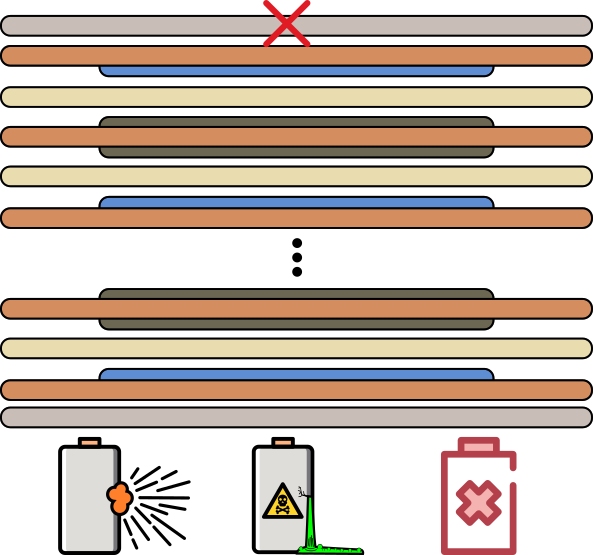
\includegraphics[width=0.2\textwidth]{failure_modes/failure_mode_pouch.png}}
    &\makecell{Elektrodenversagen\\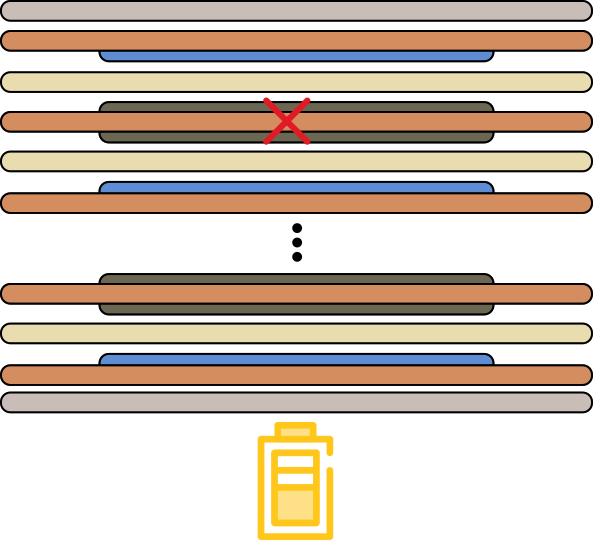
\includegraphics[width=0.2\textwidth]{failure_modes/failure_mode_electrode.png}}
    &\makecell{Separatorversagen\\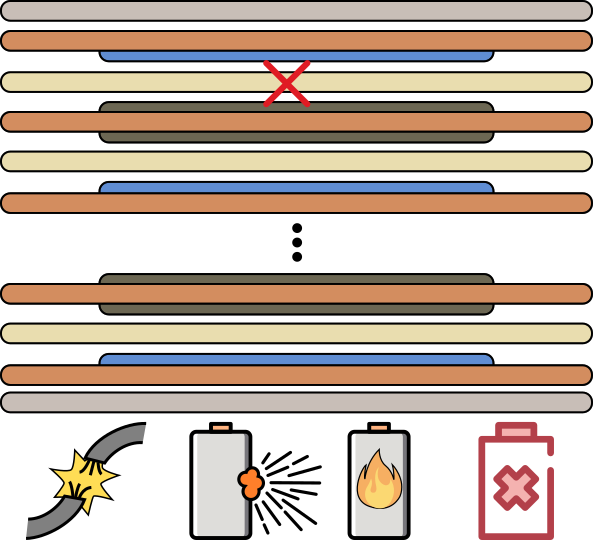
\includegraphics[width=0.2\textwidth]{failure_modes/failure_mode_separator.png}}
    \\
    \midrule
    Funktion
        & Funktionsversagen der gesamten Batterie durch austrocknen
        & Leistungsverlust der Zelle
        & Funktionsversagen der Zelle, je nach Verschaltung auch der gesamten Batterie
    \\
    Brandgefahr
        & kein Risiko
        & kein Risiko
        & Flammenbildung durch Überhitzung
    \\
    Gesundheit
        & hohes Risiko durch austretendes Elektrolyt
        & kein Risiko
        & kein zusätzliches Risiko
    \\
    \bottomrule
    \end{tabularx}\\
    %\noindent{\footnotesize{\textsuperscript{*} Gemessen gegenüber \ce{Li}/\ce{Li+}.}}
\end{table}%

\section{\label{sec:digitalisation}Erstellung einer Materialdatenbank für Strukturbatterien}
\chapter{Fertigung und experimentlle Erprobung von Strukturbatterien}
\section{Technolgische Realisierung}
\section{Messtechnik und Probekörper}
\section{Vorversuche}
\section{Verhalten unter Biegebelastung}
\section{Bestimmung der elektrochemischen Performanz}

\chapter{Vergleich experimenteller und simulativer Ergebnisse}
\section{Validierung der Eigenschaftsvorhersagen}

\section{Ashby Logic}

\chapter{Mögliche Anwendungen von Strukturbatterien im Leichtbau}

Strukturbatterien könnten Anwednungen in zahlreichen Bereichen auf vielseitige Art und Weise eingesetzt werden. 

\begin{table}[ht]
    \centering
    \caption{\label{tab:pot_anwendungen}Potentielle Anwendungen von Strukturbatterien für verschiedene Einsatzbereiche.}
    \begin{tabular}{m{0.2\textwidth} m{0.2\textwidth}<{\centering} m{0.4\textwidth}<{\centering} m{0.2\textwidth}}
        \toprule
        Technologischer Einsatzbereich&Teilbereiche&Anwendungsbeispiele&Quelle\\
        \midrule
        \multirow{3}*{Luftfahrt}   &Tertiärestrukturen&Entertainmentsystem und Innenverkleidungen& \\
                    &Sekundärstruktur&Trennwände und Gepäckfächer; Fahrwerkstüren; Rahmenstrukturen und Stellklappem& \\
                    &Primärstrukturen&Flugzeugrumpf und Flügelstrukturen& \\
                    %\hspace{1em}
                    \hline
        \multirow{3}*{Automobil}   &Karosserieteile&Türverkelidungen, Innenraumelemente und Sitzstrukturen&\\
                    &Sekundäre Fahrzeugstrukturen&Armaturenebrett; Dachhimmel; Trennwände&\\
                    &Tragende Strukturen&Fahrgestell oder Karosserie&\\
                    \hline
        Innenraumelemente und Sitzstrukturen&\\
                    &Sekundäre Fahrzeugstrukturen&Armaturenebrett; Dachhimmel; Trennwände&\\
                    &Tragende Strukturen&Fahrgestell oder Karosserie&\\
        \bottomrule
    \end{tabular}
\end{table}

\section{Roadmap}
Eine Abschätzung 


\section{Potenzial für den Flugzeugkabineninnenraum}

\begin{figure}[!h]
	%\raggedleft
		%\def\svgwidth{\columnwidth}
        \center
		\includegraphics[width=0.8\textwidth, angle=0]{Abbildungen/06_Leichtbau/cabine_usecase.pdf}
		\caption{\label{fig:cabin}Der Einsatz von Strukturbatterien kann in Flugzeugkabinen dazu eingesetz werden um eine kabelose Stromversorgung am Passagiersitz zu ermöglichen, was nicht nur Kabel einsparrt, sonder auch bei der Gewichtsverteilung hilft.}
\end{figure}

\section{Potenzial für die mobile Robotik}

\begin{figure}[!h]
	%\raggedleft
		%\def\svgwidth{\columnwidth}
        \center
		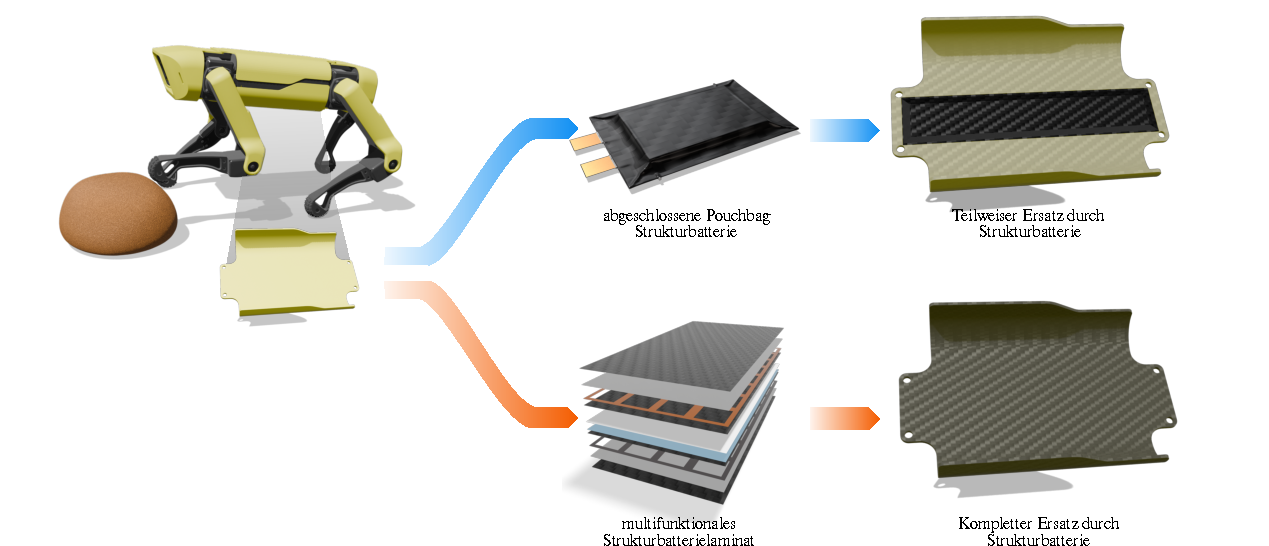
\includegraphics[width=0.99\textwidth, angle=0]{Abbildungen/06_Leichtbau/dog_robot_sb_study.pdf}
		\caption{\label{fig:robot_dog}In der mobilen Robotik können Strukturbatterien durch Integration bisher primaär Lastentragende Komponenten Integirert werden, um die Reichweite zu erhöhen.}
\end{figure}

\include{Kapitel/07_Zusammenfassung}

%Literaturverzeichnis und Datenbank einfügen
\nocite{} %\nocite{*} --> alle in der Datenbank existierenden Einträge werden bearbeitet; ohne * --> nur die verwendeten werden aufgeführt
\bibliographystyle{plaindin_mod} %Aussehen des Literaturverzeichnisses
\bibliography{Literatur_Diss} % Einbinden der Literaturdatenbank <yyyymmdd_Literatur.bib>
%\printbibliography
\appendix
\include{Kapitel/09_Anhang}

\cleardoublepage
\include{Kapitel/10_Lebenslauf}

\end{document}

